% !TeX encoding = UTF-8
% !TeX program = pdflatex
% !TeX spellcheck = en_EN
\documentclass[binding=0.6cm,noexaminfo]{sapthesis}
\usepackage{microtype} \usepackage[english]{babel}
\usepackage[utf8]{inputenc} \usepackage{hyperref}
\usepackage{array} \usepackage{listings}
\usepackage{xcolor}
\usepackage{graphicx}
\usepackage{amssymb}
\usepackage{pifont}
\newcommand{\cmark}{\ding{51}}%
\newcommand{\xmark}{\ding{55}}%
\graphicspath{ {./images/} }

\usepackage[style=numeric]{biblatex}
\addbibresource{bibliography.bib}

\definecolor{codegreen}{rgb}{0,0.6,0}
\definecolor{codegray}{rgb}{0.5,0.5,0.5}
\definecolor{codeorange}{rgb}{1,0.6,0.2}
\definecolor{backcolour}{rgb}{0.95,0.95,0.92}
\definecolor{green}{rgb}{0,0.7,0}
\definecolor{red}{rgb}{0.9,0,0}

\lstdefinestyle{mystyle}{
    backgroundcolor=\color{backcolour},   
    commentstyle=\color{codegreen},
    keywordstyle=\bf\color{black},
    numberstyle=\tiny\color{codegray},
    stringstyle=\color{codeorange},
    basicstyle=\ttfamily\footnotesize,
    breakatwhitespace=false,         
    breaklines=true,                 
    captionpos=b,                    
    keepspaces=true,                 
    numbers=left,                    
    numbersep=5pt,                  
    showspaces=false,                
    showstringspaces=false,
    showtabs=false,                  
    tabsize=2
}

\lstset{style=mystyle}

\hypersetup{pdftitle={Internship Report: MQTT over TLS Security Assessment},pdfauthor={Radek Patrick Di Luca}}
\title{Internship Report: MQTT over TLS Security Assessment} \author{Radek Patrick Di Luca}
\IDnumber{1803854}
\course{Corso di laurea triennale in Informatica erogato in modalità Teledidattica}
\courseorganizer{Facoltà di Ingegneria dell’Informazione, Informatica e Statistica} \AcademicYear{2023/2024}
\advisor{Prof. Angelo Spognardi}
\customadvisorlabel{Responsabile}
\authoremail{diluca.1803854@studenti.uniroma1.it}
\copyyear{2023}
\thesistype{Relazione di Tirocinio}
\begin{document}
\frontmatter
\maketitle
\tableofcontents
\mainmatter
\chapter{Introduction}
\section{Problem Definition}
The aim of this internship work was to assess the security of the TLS Protocol implementation of some of the main MQTT Broker Libraries that can be found in the IT community. Some faults in the Application layer Protocol (MQTT) of some of these libraries were found by my colleague Edoardo Di Paolo during his Internship work \cite{mqttpaper}, so the hypothesis was that these libraries might very well have some faults in the Transport layer Protocol (TLS) too.
Therefore, through the generation of some forged TLS Certificates and the definition of a Suite of Automated Unit Tests, the goal was to expose vulnerabilities in these libraries, or validate their implementation as secure.

\section{Related Works}
As it was just stated, the main inspiration for this work has been the article published by my colleague Edoardo Di Paolo \cite{mqttpaper}, which gave us clear information on the publish-subscribe communication paradigm of the MQTT Protocol and on which libraries to test, finally focusing our efforts on the \textit{Mosquitto}, \textit{HiveMQ}, \textit{Moquette}, \textit{EMQX} and \textit{Aedes} MQTT Broker Libraries. The article \cite{mqttpaper} also helped us designing our communication Test Environment, which is later discussed in \textit{Chapter/Section (TODO)}.

On top of that, the research led by Stanford and Texas at Austin Universities on SSL Certificate Validation in Non-Browser Software \cite{sslvalidation} helped us targeting possible MQTT over TLS Implementation Faults, namely \textit{Chain Of Trust Verification}, \textit{Hostname Verification} and \textit{X.509 Extension Verification}. The research \cite{sslvalidation} also pointed us towards the official RFCs \cites{rfc2818}{rfc5280}{rfc8446} which contain more extensive information regarding TLS Certificate Validation. All these pieces of information allowed us to formally define the TLS Vulnerabilities and Unit Test Suite, described respectively in \textit{Chapter/Section (TODO)} and \textit{Chapter/Section (TODO)}.

Finally, the article published by University of Padua and the Technical University of Denmark on the design of an SSL Validation Proxy named MITHYS \cite{mithys} exhibits how similar TLS Implementation Faults could be found in some widely spread Mobile Application Software.

\section{Key Concepts}
For the sake of this report, we will be using some core concepts that are critical to understanding the Internship work.

\subsection{MQTT}
MQTT, also known as Message Queuing Telemetry Transport, is a lightweight protocol used on the Application Layer of the TCP/IP stack. MQTT is an alternative to the widely spread HTTP, and it’s mainly used for connectivity to and from Internet of Things devices, due to the lightweight nature of the protocol and due to the low memory availability of the above mentioned IoT devices.
Since the MQTT protocol is by nature a lightweight protocol, it does not feature many security capabilities, so it must rely on the security checks made by the layer immediately below MQTT, the Transport layer, via SSL/TLS.
We can see here a representation of a typical message exchange via the MQTT protocol:

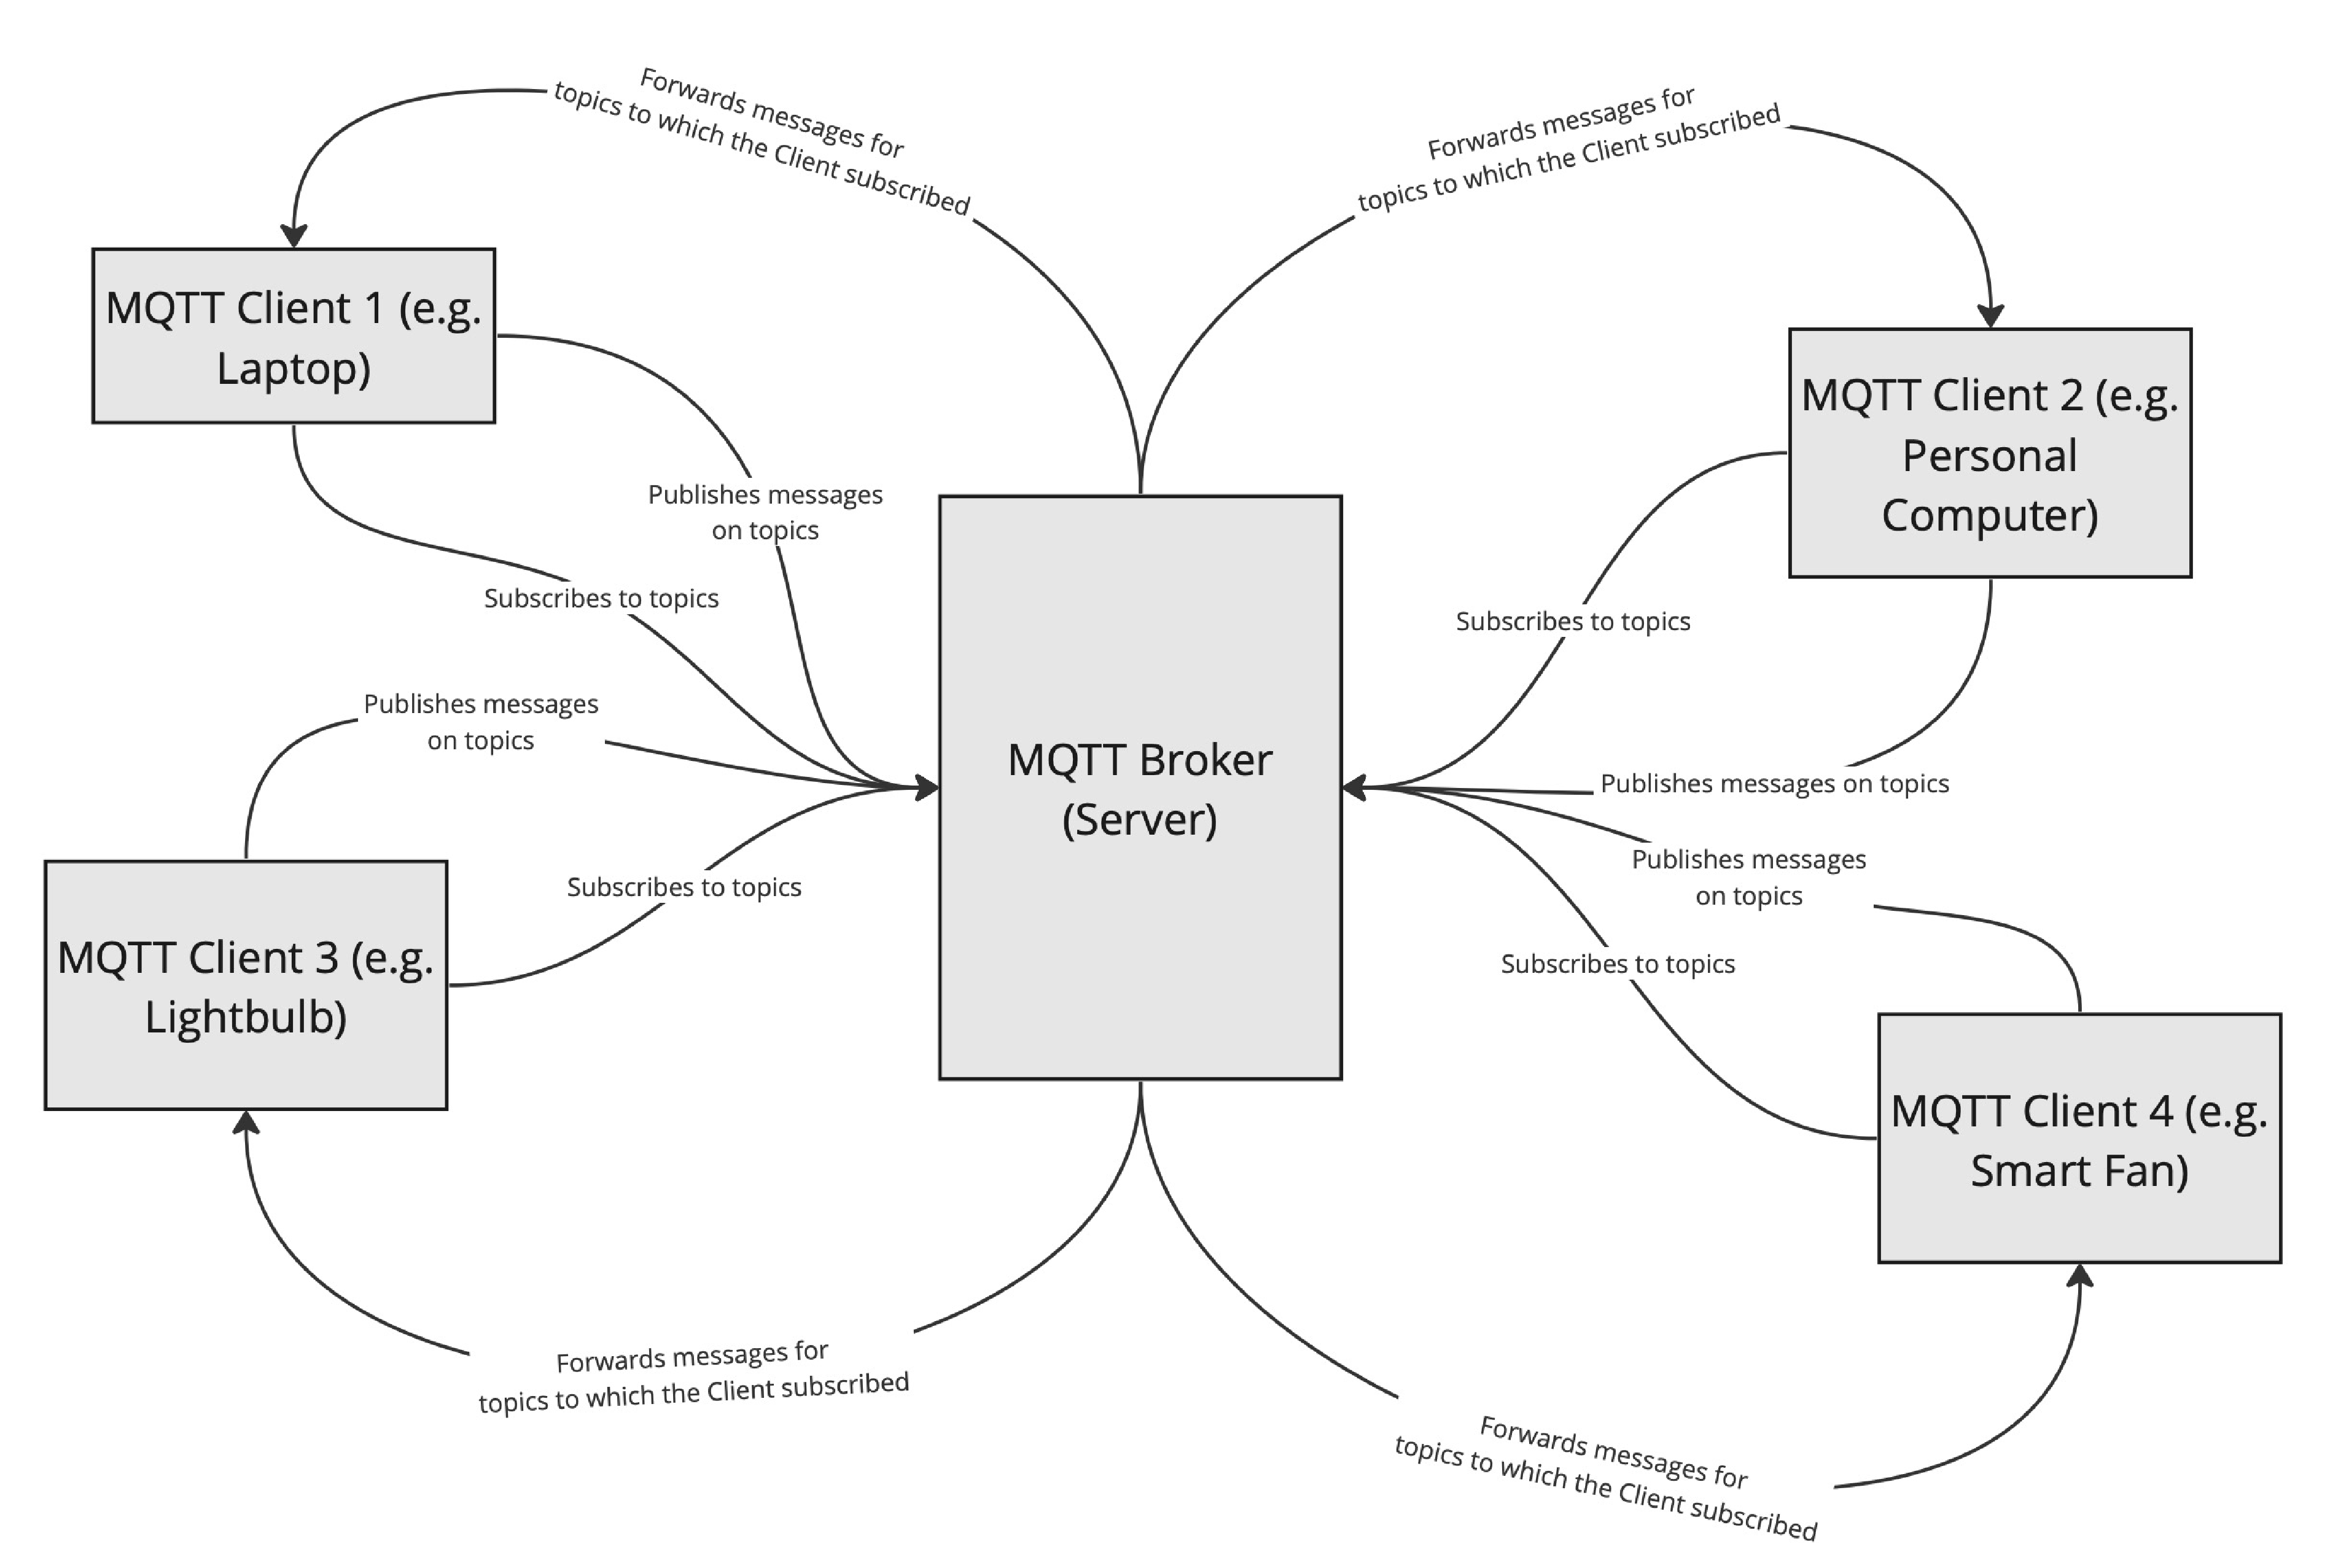
\includegraphics[width=13cm]{MQTT}

The exchange of information is mainly done through the publish/subscribe paradigm:
\begin{itemize}
	\item \textbf{subscribe}: an MQTT Client subscribes to one or more topics. Each topic is identified by a unique string and after subscribing to the topic(s), the MQTT Client will be in a `listening' state, receiving any new messages that will be published on the topic(s).
	\item \textbf{publish}: an MQTT Client publishes a message to a topic. Each topic is identified by a unique string, and by publishing the message, any Client that was subscribed to the topic will receive the published message.
\end{itemize}

\subsection{SSL/TLS}
SSL, also known as Secure Sockets Layer, is a protocol used on the Transport Layer of the TCP/IP stack, to provide security in the form of confidentiality, integrity and authenticity to one or both parties involved in the message exchange. In fact, SSL consists mainly of a Handshake phase, in which the client and server negotiate the parameters that will be used to establish the security of the following communication. During this Handshake phase, it is possible to negotiate whether the security is one-way (only the server is authenticated towards the client) or both ways (also known as mutual SSL, mutual TLS or abbreviated, mTLS).

\subsection{Certificate Authority}
A Certificate Authority, abbreviated CA, is a secure third party who is trusted by both TLS server and TLS client. In general, the client trusts the CA to certify that the server is who they claim to be. In mutual TLS, the CA is also used by the server, to certify that the client is who they claim to be.

\section{TLS Vulnerabilities}
One of the main pieces of work done for this Internship was to define the ways in which an Attacker could possibly exploit a badly implemented TLS connection. Therefore, referencing the specifications RFC 2818 \cite{rfc2818}, RFC 8446 \cite{rfc8446} and RFC 5280 \cite{rfc5280}, the following list of validations an MQTT Broker Library should implement was produced:

\begin{itemize}
	\item \textbf{Chain of trust}: the certificate has to be either signed by a root Certificate Authority, or it has to have a linked list of references to various Certificate Authorities, up to a root node certificate self-signed by a root Certificate Authority. In this linked list, the certificate of every issuing Certificate Authority has to be signed by the Certificate Authority immediately above it. Validating this check led us to define \textit{Test Cases 1, 2, 3, and 9}.
	\item \textbf{Hostname}: the \textit{Common Name} field should match the identifier of the entity to which we’re connecting (server). Validating this check led us to define \textit{Test Cases 4 and 10}.
	\item \textbf{(Recursive) Expiration}: the \textit{Not Valid Before} and \textit{Not Valid After} fields contain information on the timestamps that delimit the interval in which the certificate should be accepted as valid. The Library should check that today's date is contained within that interval. This is valid also recursively for the Certificates of the issuing Certificate Authorities throughout the chain of trust. Validating this check led us to define \textit{Test Cases 5 and 7}.
	\item \textbf{Public key}: the \textit{Public Key Info > Public Key} field should match the information provided by the Certificate Authority. This public key will be used to encrypt all the upcoming communication, so using the correct public key is essential. Validating this check led us to define \textit{Test Cases 6 and 11}.
	\item \textbf{X.509 Certificate Extension}: the \textit{Certificate Extensions} should not contain information that would impair the validity of the Certificate itself. In our example, in \textit{Test Case 8}, the Certificate used by the MQTT Server should not be flagged as "Client Only" in the Certificate Extensions, and the tested Library should check for these fields to be valid.
	\item \textbf{Downgrade attack}: some attackers might try pretending that the latests versions of TLS are not supported by one of the two communicating parties, or they could also pretend that the set of supported ciphers is limited to only easily breakable ciphers, for example based on 512 bit-long cipher keys. This is why it’s important to support only the versions of TLS that are still considered secure, and it’s important to restrict the set of supported ciphers to only implementation-strong ciphers. This known vulnerability led us to test RouterOS for weak ciphers. This will be described later in \textit{Chapter/Section (TODO)}.
\end{itemize}

\chapter{Test Suite}
To test the MQTT Broker Libraries, a Unit Test Suite was formally defined, with a series of descriptions and assertions made. The Unit Tests are defined following the Triangulation technique, which means that the Test Suite should assert both the valid scenarios in which the connection should be established and the illegal scenarios in which the connection should be rejected. Hence the Tests are defined as follows:
\begin{enumerate}
	\item Test Case 1 - Legal Connection
	\item Test Case 2 - Self Signed Attacker
	\item Test Case 3 - Self Signed Attacker's Fake CA
	\item Test Case 4 - Alteration 1 (Common Name)
	\item Test Case 5 - Alteration 2 (Expiration Date)
	\item Test Case 6 - Alteration 3 (Public Key)
	\item Test Case 7 - Expired CA (Alteration 4)
	\item Test Case 8 - Certificate Extension
	\item Test Case 9 - Longer Chain Of Trust Legal Connection
	\item Test Case 10 - Altered Intermediate CA Common Name
	\item Test Case 11 - Altered Intermediate CA Public Key
\end{enumerate}
Note: The tested libraries are set up as MQTT Broker, or MQTT Server. The Client, which asserts the outcome of the test, always uses the Mosquitto command line tools to connect to the Server.

\section{Test Case 1 - Legal Connection}
This Test Case is set up by configuring the MQTT Broker Library with a valid TLS Certificate signed by the real Certificate Authority. The Tester Client connects to the server checking the Server TLS Certificate against the real Certificate Authority’s Certificate. The table of the Unit Test is as follows:

\begin{center}
\begin{tabular}{| p{6cm} | p{6cm} |}
\hline
Intruder Access Capabilities & None \\
\hline
Intruder’s Attack description & This test case represents the happy path with no intruder attack. \\
\hline
State of TLS Certificate & The TLS Certificate we use for this test is exactly the Server’s Certificate. \\
\hline
State of Certificate’s Signature & The signature is \textbf{\textit{valid}} \\
\hline
Assertion & The Library should \textbf{\textit{accept}} the connection when a client tries connecting to the MQTT Library configured with this certificate. \\
\hline
\end{tabular}
\end{center}

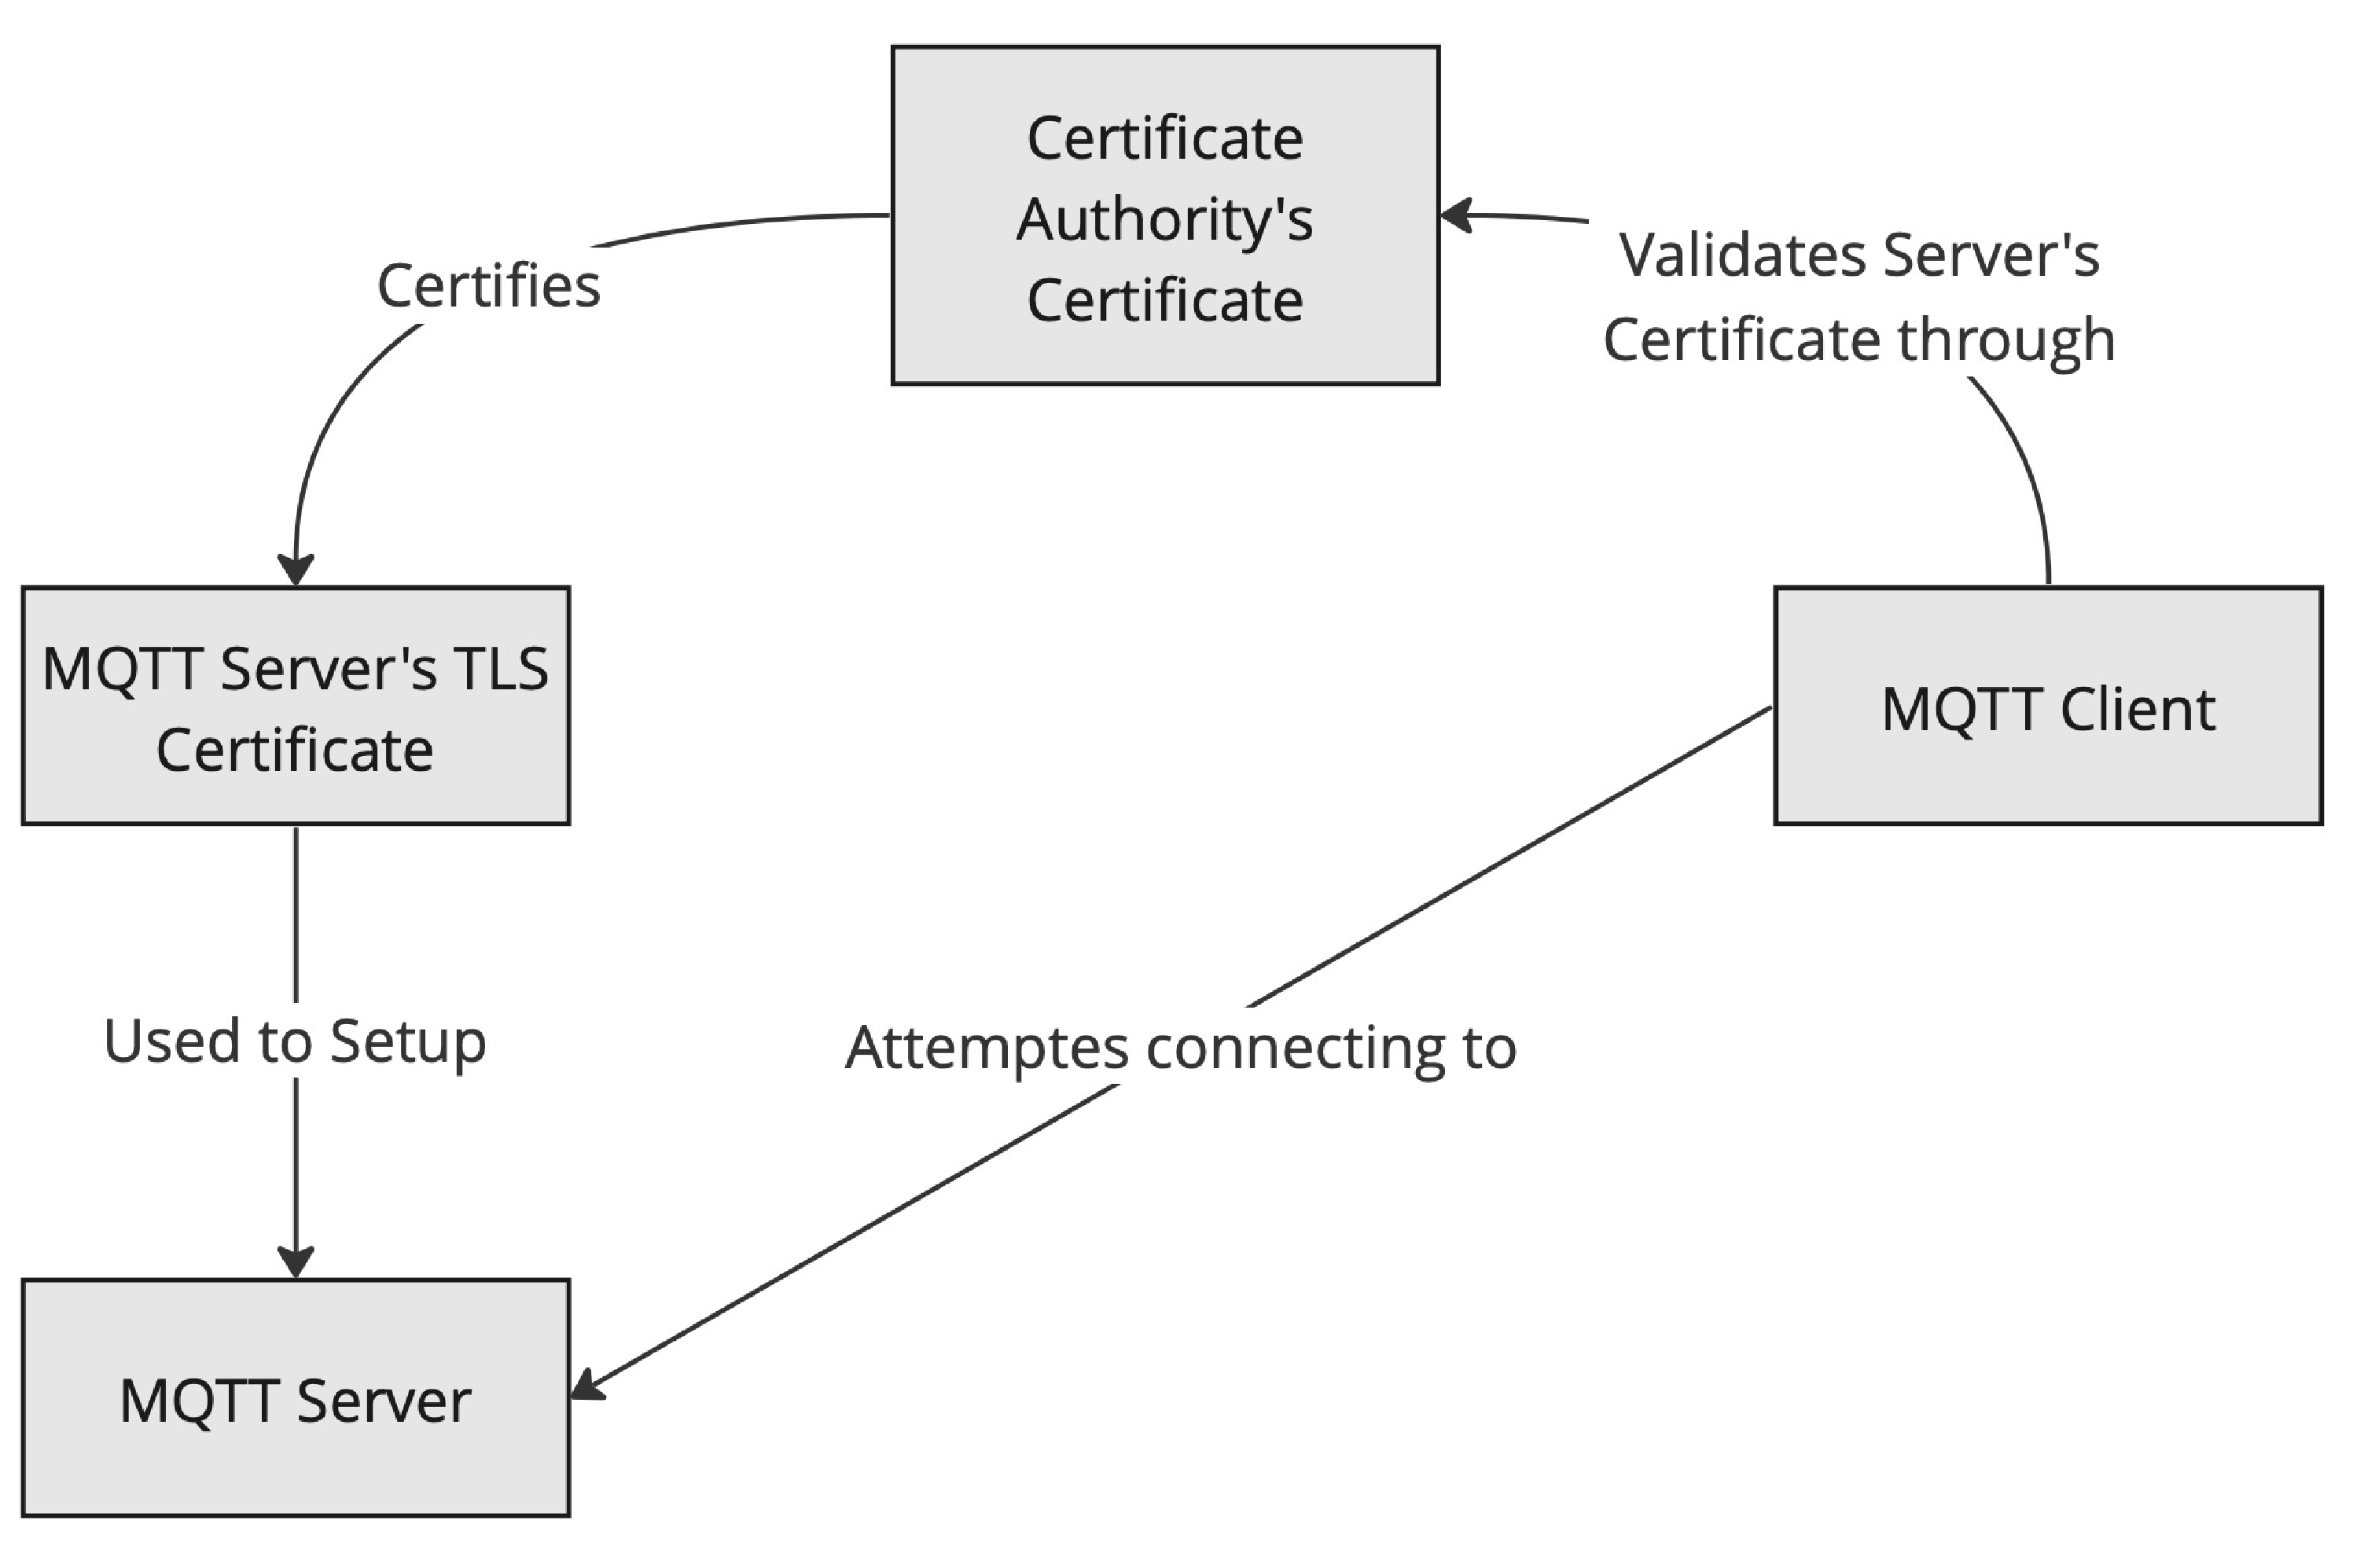
\includegraphics[width=13cm]{TC1}

\section{Test Case 2 - Self Signed Attacker}
This Test Case is set up by configuring the MQTT Broker Library with a forged self-signed TLS Certificate. The Tester Client connects to the server checking the Server TLS Certificate against the real Certificate Authority’s Certificate. The table of the Unit Test is as follows:

\begin{center}
\begin{tabular}{| p{6cm} | p{6cm} |}
\hline
Intruder Access Capabilities & The Intruder impersonates an MQTT Server during the TLS Handshake phase. \\
\hline
Intruder’s Attack description & The Intruder creates a self-signed certificate and uses it to configure the MQTT Library. \\
\hline
State of TLS Certificate & The TLS Certificate is self-signed by the attacker, so any field can be completely different from the Server’s Certificate. \\
\hline
State of Certificate’s Signature & The signature is \textbf{\textit{valid}} \\
\hline
Assertion & The Library should \textbf{\textit{reject}} the connection when a client tries connecting to the MQTT Library configured with this certificate. \\
\hline
\end{tabular}
\end{center}

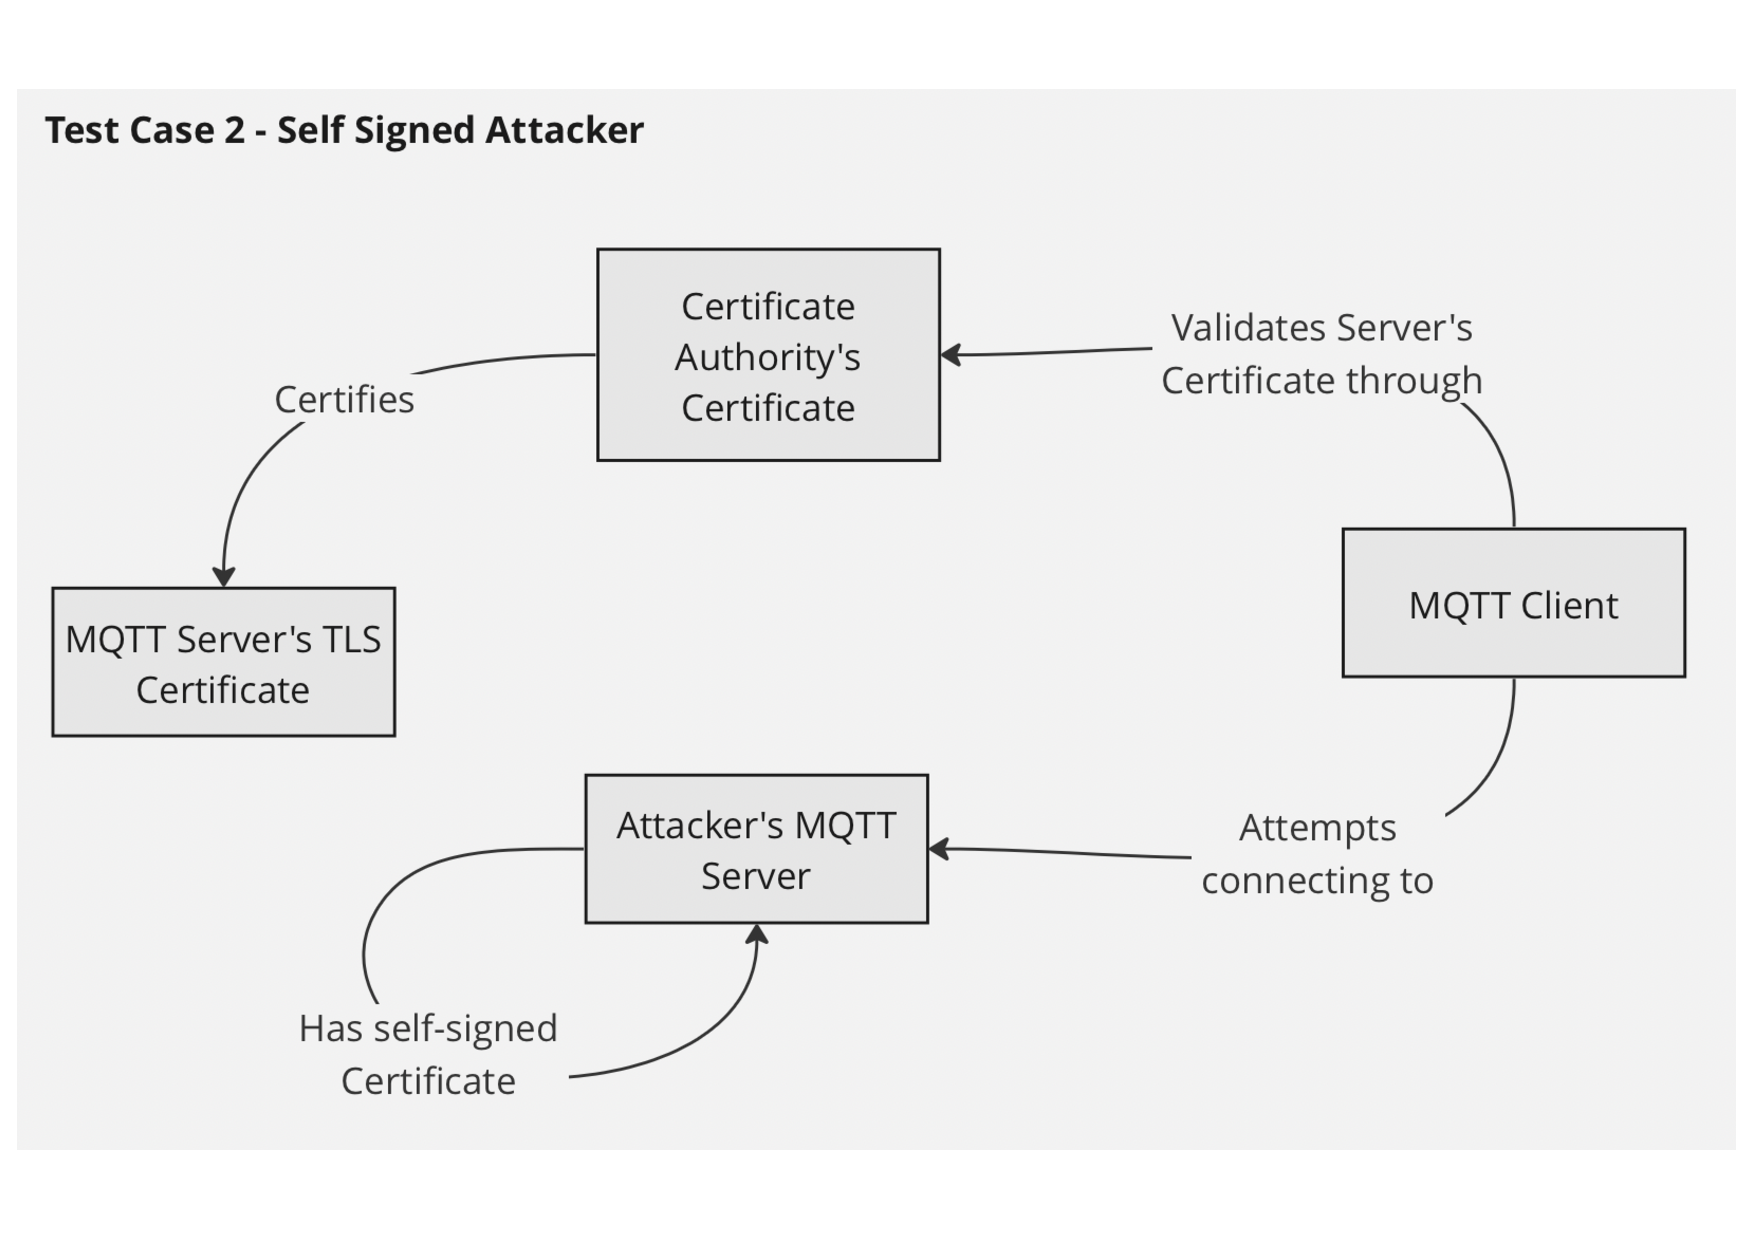
\includegraphics[width=13cm]{TC2}

\section{Test Case 3 - Self Signed Attacker's Fake CA}
This Test Case is set up by configuring the MQTT Broker Library with a forged TLS Certificate signed by a forged Root Certificate Authority. The Tester Client connects to the server checking the Server TLS Certificate against the real Certificate Authority’s Certificate. The table of the Unit Test is as follows:

\begin{center}
\begin{tabular}{| p{6cm} | p{6cm} |}
\hline
Intruder Access Capabilities & The Intruder impersonates an MQTT Server during the TLS Handshake phase. \\
\hline
Intruder’s Attack description & The Intruder imitates the Server Certificate’s chain of trust, creating their own root Certificate Authority and using it to sign their certificate. Then they use their certificate to configure the MQTT Library. \\
\hline
State of TLS Certificate & The TLS Certificate is imitating the Server Certificate, but it’s signed by the Attacker’s fake Certificate Authority. \\
\hline
State of Certificate’s Signature & The signature is \textbf{\textit{valid}} \\
\hline
Assertion & The Library should \textbf{\textit{reject}} the connection when a client tries connecting to the MQTT Library configured with this certificate. \\
\hline
\end{tabular}
\end{center}

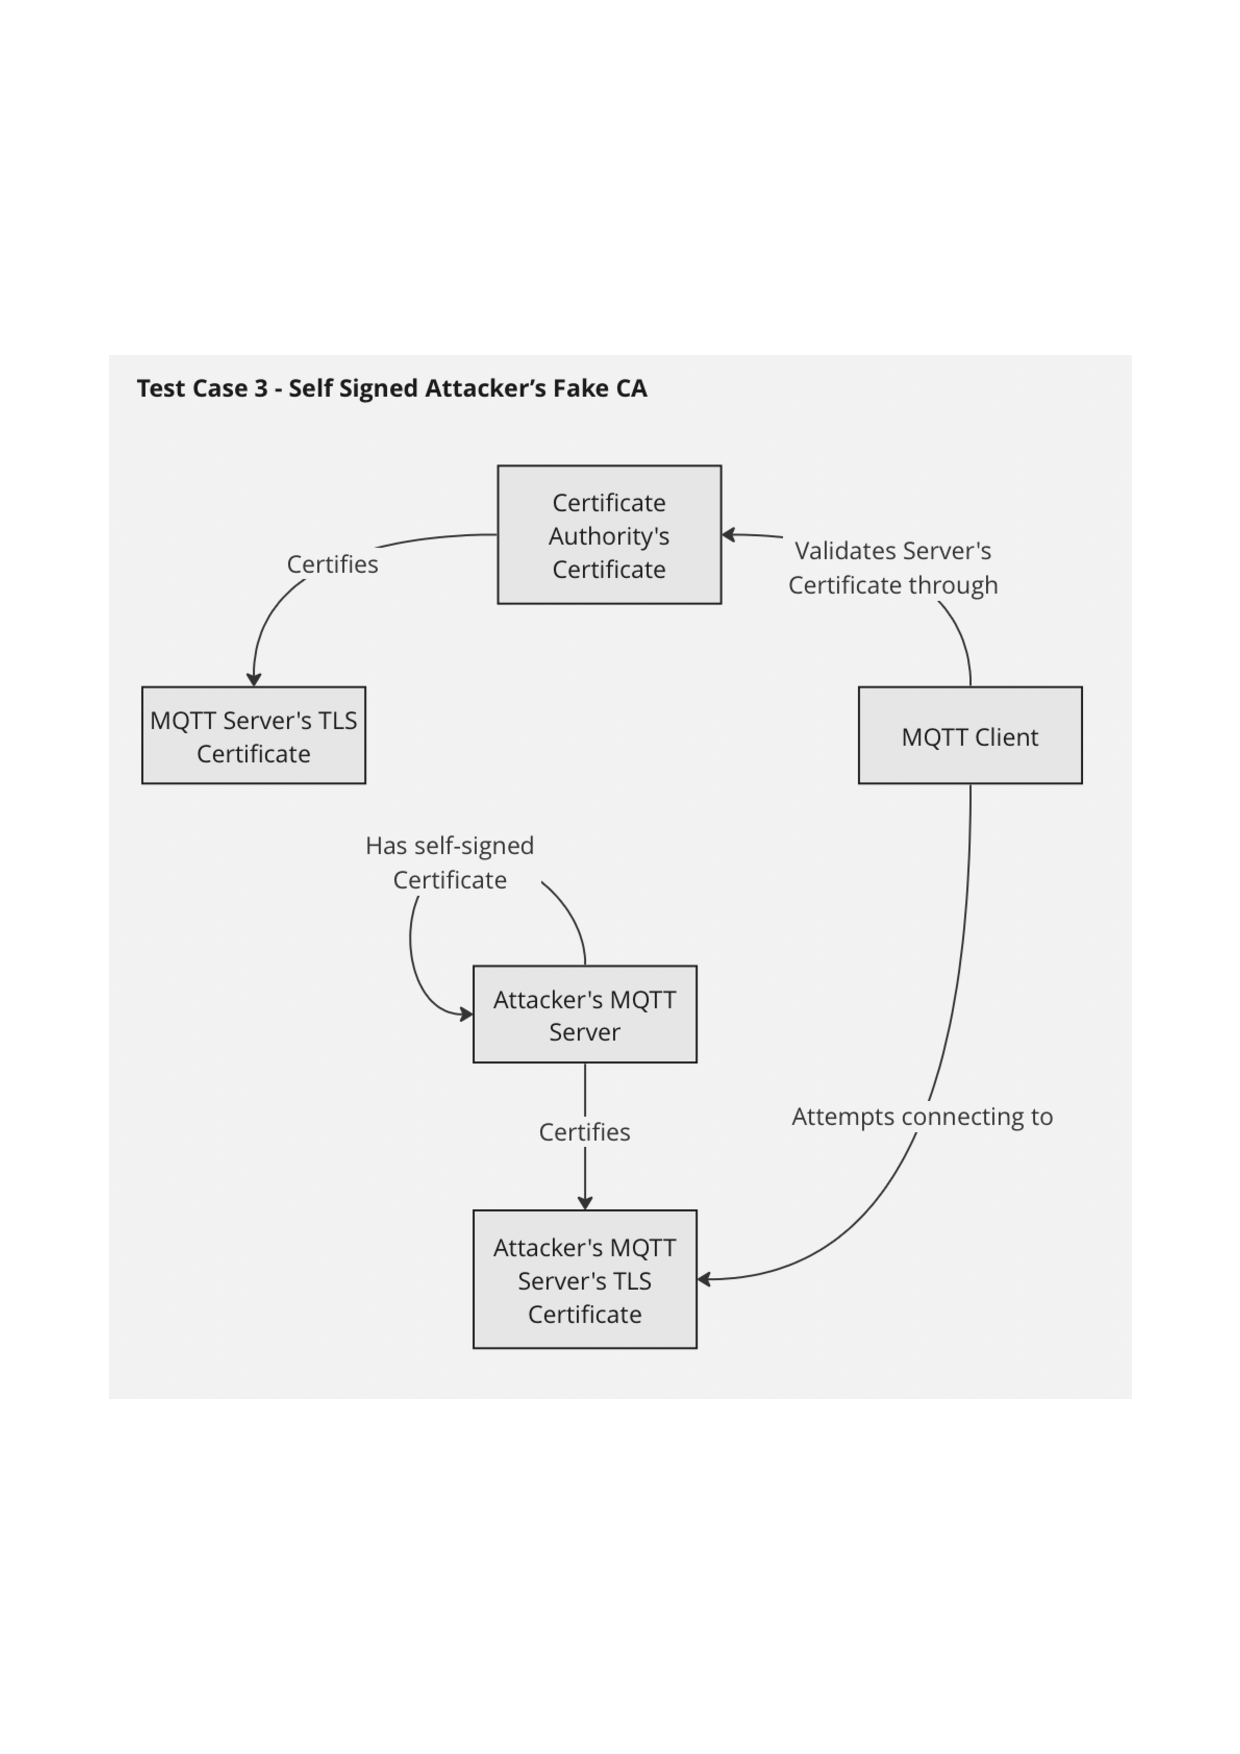
\includegraphics[width=13cm]{TC3}

\newpage
\section{Test Case 4 - Alteration 1 (Common Name)}
This Test Case is set up by configuring the MQTT Broker Library with an altered TLS Certificate signed by the real Certificate Authority. The intruder alters the Common Name field, therefore the signature is compromised because the Server Certificate has been tampered with. The Tester Client connects to the server checking the Server TLS Certificate against the real Certificate Authority’s Certificate. The table of the Unit Test is as follows:

\begin{center}
\begin{tabular}{| p{6cm} | p{6cm} |}
\hline
Intruder Access Capabilities & The Intruder impersonates an MQTT Server during the TLS Handshake phase. \\
\hline
Intruder’s Attack description & The Intruder alters the Common Name field of the Server Certificate, replacing it with their own Common Name. Then they use the altered certificate to configure the MQTT Library. \\
\hline
State of TLS Certificate & The TLS Certificate is equal to the Server Certificate except for the Common Name field. \\
\hline
State of Certificate’s Signature & The signature is \textbf{\textit{not}} valid \\
\hline
Assertion & The Library should \textbf{\textit{reject}} the connection when a client tries connecting to the MQTT Library configured with this certificate. \\
\hline
\end{tabular}
\end{center}

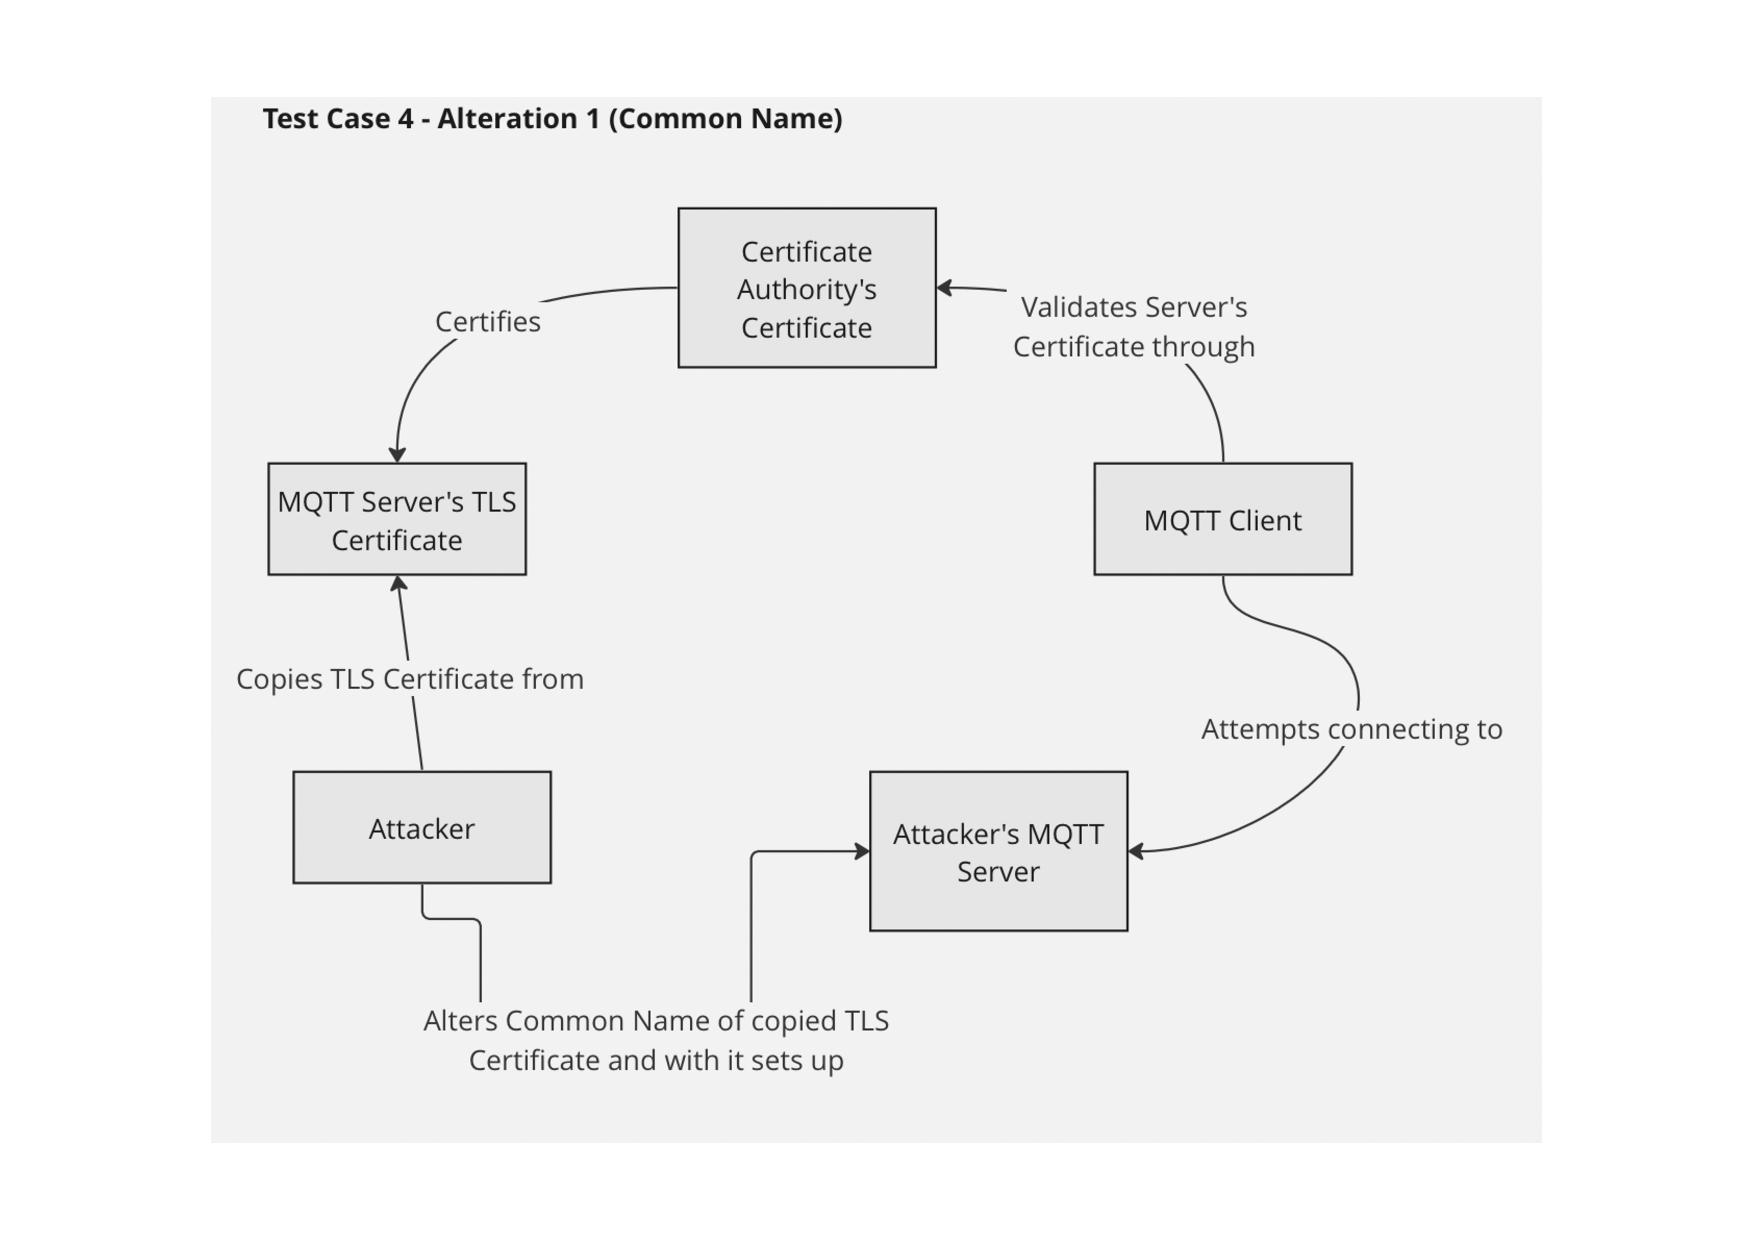
\includegraphics[width=12cm]{TC4}

\newpage
\section{Test Case 5 - Alteration 2 (Expiration Date)}
This Test Case is set up by configuring the MQTT Broker Library with an altered expired TLS Certificate signed by the real Certificate Authority. The intruder alters the Not Valid After field, therefore the signature is compromised because the Server Certificate has been tampered with. The Tester Client connects to the server checking the Server TLS Certificate against the real Certificate Authority’s Certificate. The table of the Unit Test is as follows:

\begin{center}
\begin{tabular}{| p{6cm} | p{6cm} |}
\hline
Intruder Access Capabilities & The Intruder has access to an old expired Server Certificate \\
\hline
Intruder’s Attack description & The Intruder alters the expiration date of the expired Server Certificate, making it valid for the current date. Then the Intruder tries  to configure the MQTT Library with the altered Certificate. \\
\hline
State of TLS Certificate & The TLS Certificate is the expired Server Certificate, but the Not Valid After field has been tampered with. \\
\hline
State of Certificate’s Signature & The signature is \textbf{\textit{not}} valid \\
\hline
Assertion & The Library should \textbf{\textit{reject}} the connection when a client tries connecting to the MQTT Library configured with this certificate. \\
\hline
\end{tabular}
\end{center}

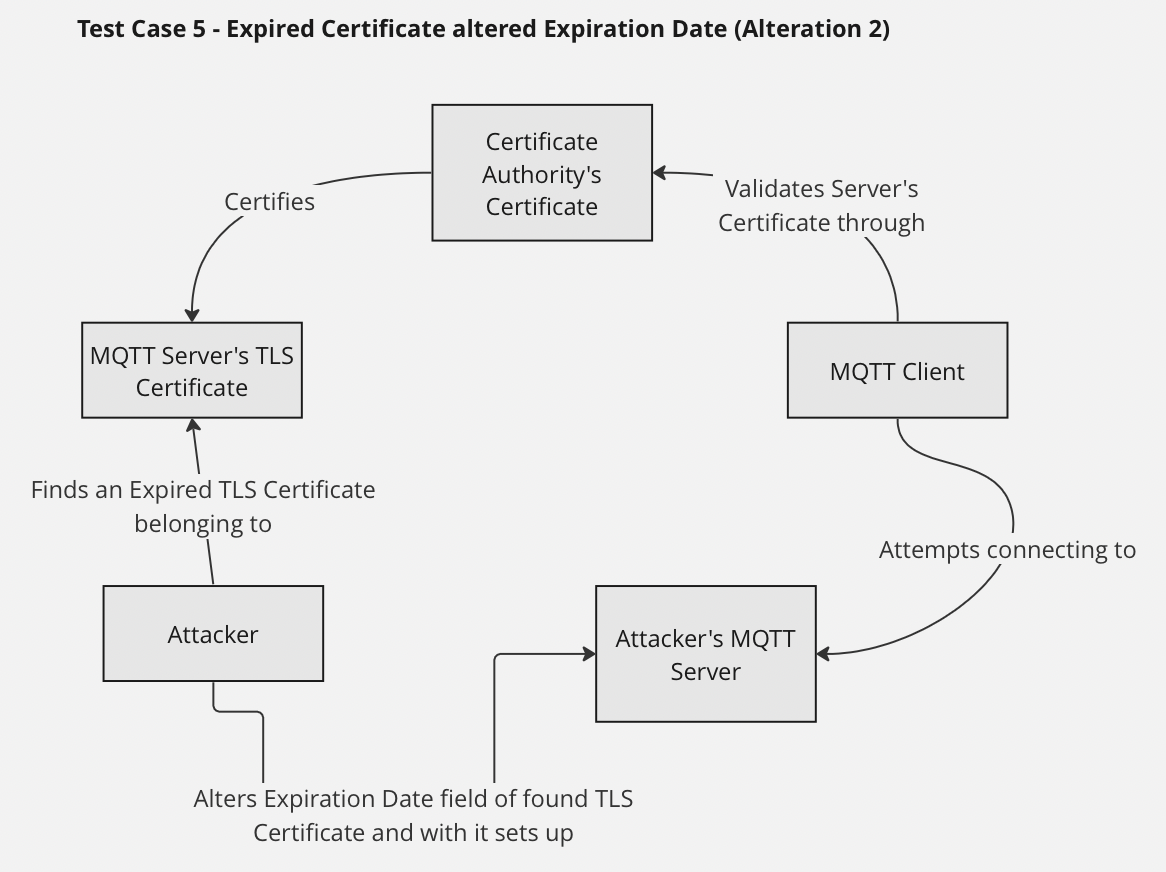
\includegraphics[width=13cm]{TC5}

\section{Test Case 6 - Alteration 3 (Public Key)}
This Test Case is set up by configuring the MQTT Broker Library with an altered TLS Certificate signed by the real Certificate Authority. The intruder replaces the contents of the Public Key field with their own Public Key, therefore the signature is compromised because the Server Certificate has been tampered with. The Tester Client connects to the server checking the Server TLS Certificate against the real Certificate Authority’s Certificate. The table of the Unit Test is as follows:

\begin{center}
\begin{tabular}{| p{6cm} | p{6cm} |}
\hline
Intruder Access Capabilities & The Intruder impersonates an MQTT Server during the TLS Handshake phase. \\
\hline
Intruder’s Attack description & The Intruder alters the Public Key Info > Public Key field of the Server Certificate, replacing it with their own Public Key. Then they use the altered certificate to configure the MQTT Library. \\
\hline
State of TLS Certificate & The TLS Certificate is equal to the Server Certificate except for the Public Key field. \\
\hline
State of Certificate’s Signature & The signature is \textbf{\textit{not}} valid \\
\hline
Assertion & The Library should \textbf{\textit{reject}} the connection when a client tries connecting to the MQTT Library configured with this certificate. \\
\hline
\end{tabular}
\end{center}

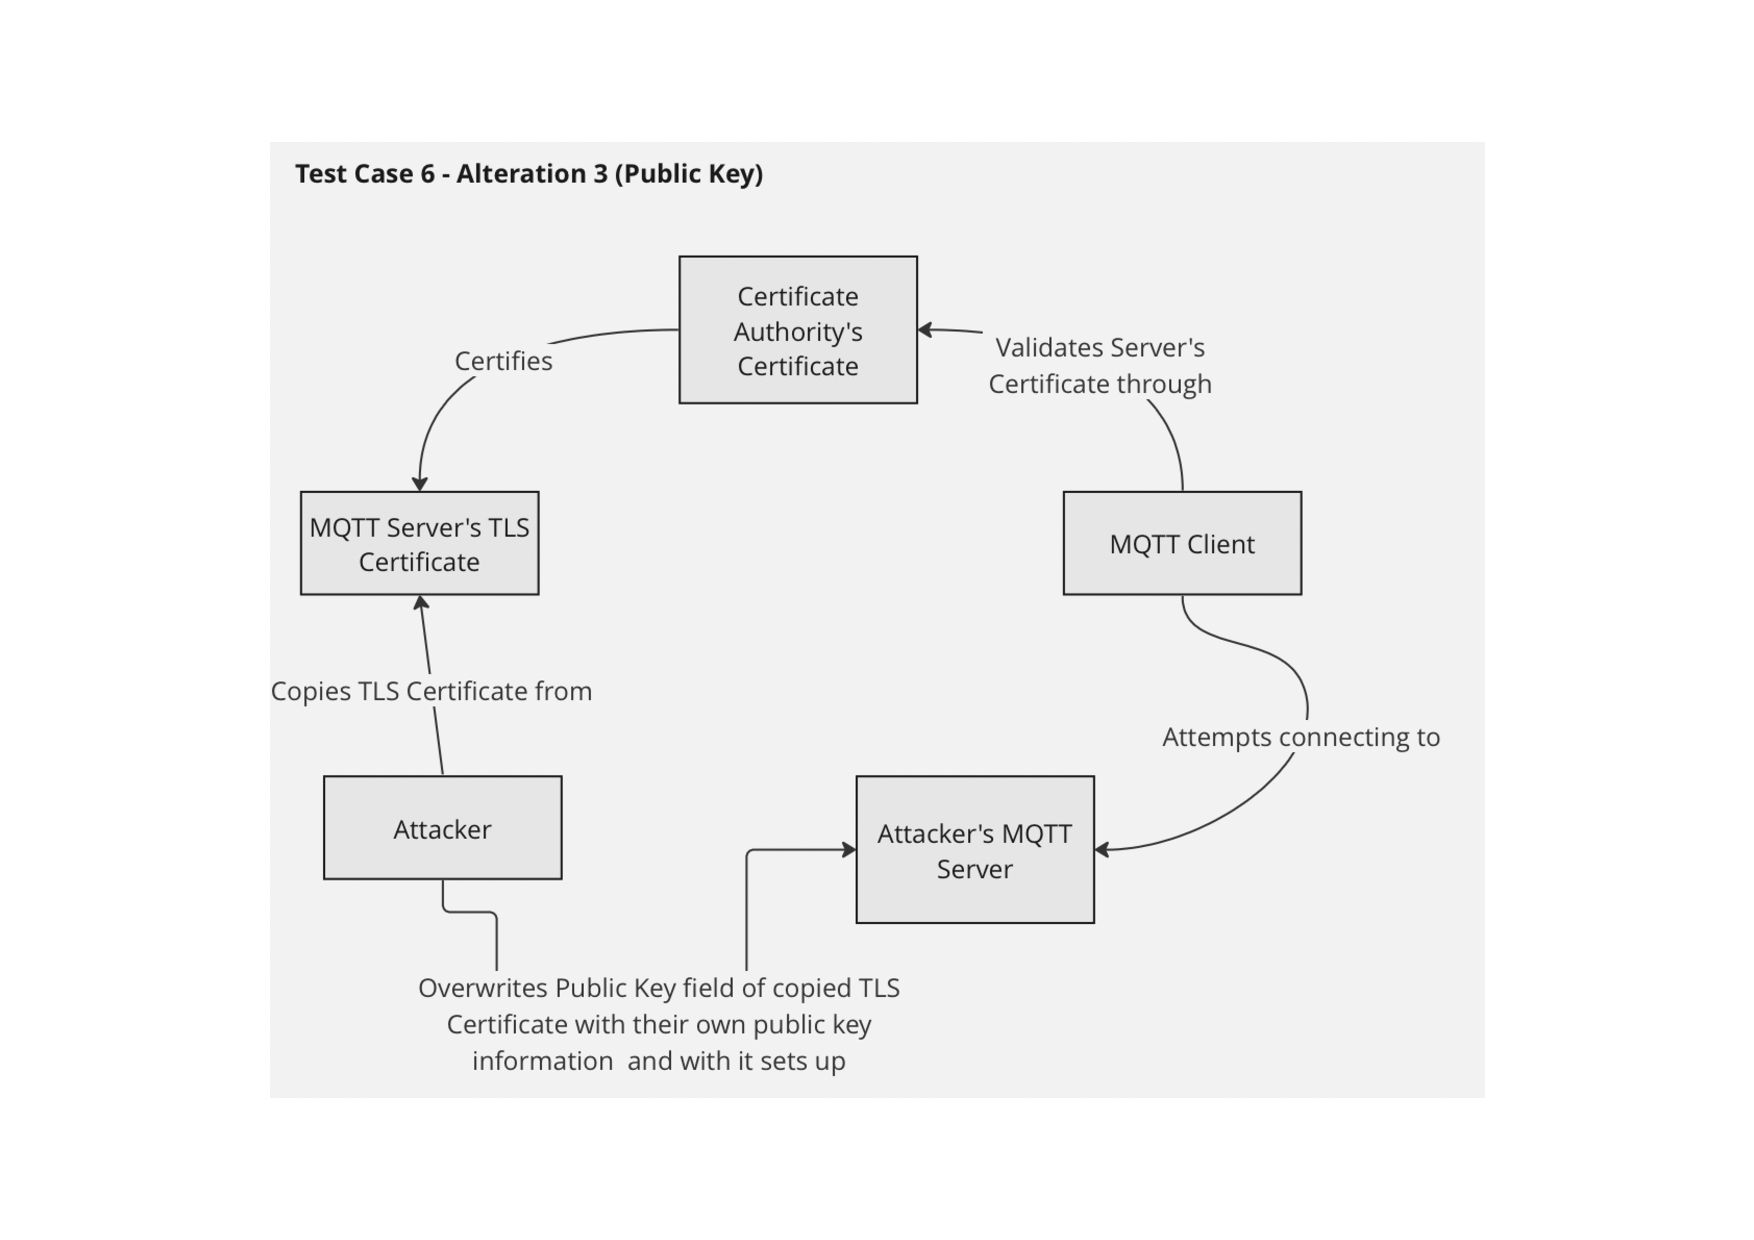
\includegraphics[width=12cm]{TC6}

\newpage
\section{Test Case 7 - Expired CA (Alteration 4)}
This Test Case is set up by configuring the MQTT Broker Library with a forged TLS Certificate signed by an expired (real) Certificate Authority. This test represents a scenario in which the Intruder manages to decrypt the Certificate Authority’s Public Key over a long period of time, during which the Client under attack is not updated with a new CA Certificate. Because of this, the Tester Client in this Test Case connects to the server checking the Server TLS Certificate against the expired Certificate Authority’s Certificate. The table of the Unit Test is as follows:

\begin{center}
\begin{tabular}{| p{6cm} | p{6cm} |}
\hline
Intruder Access Capabilities & The Intruder has access to an old expired Certificate Authority Root or Intermediate Certificate \\
\hline
Intruder’s Attack description & The Intruder tries using the formerly valid, but now expired, Certificate Authority Certificate, to sign their own certificate. Then they try using this certificate to configure the MQTT Library. \\
\hline
State of TLS Certificate & The TLS Certificate is a completely different certificate from the Server Certificate. \\
\hline
State of Certificate’s Signature & The signature is \textbf{\textit{valid}} \\
\hline
Assertion & The Library should \textbf{\textit{reject}} the connection when a client tries connecting to the MQTT Library configured with this certificate. \\
\hline
\end{tabular}
\end{center}

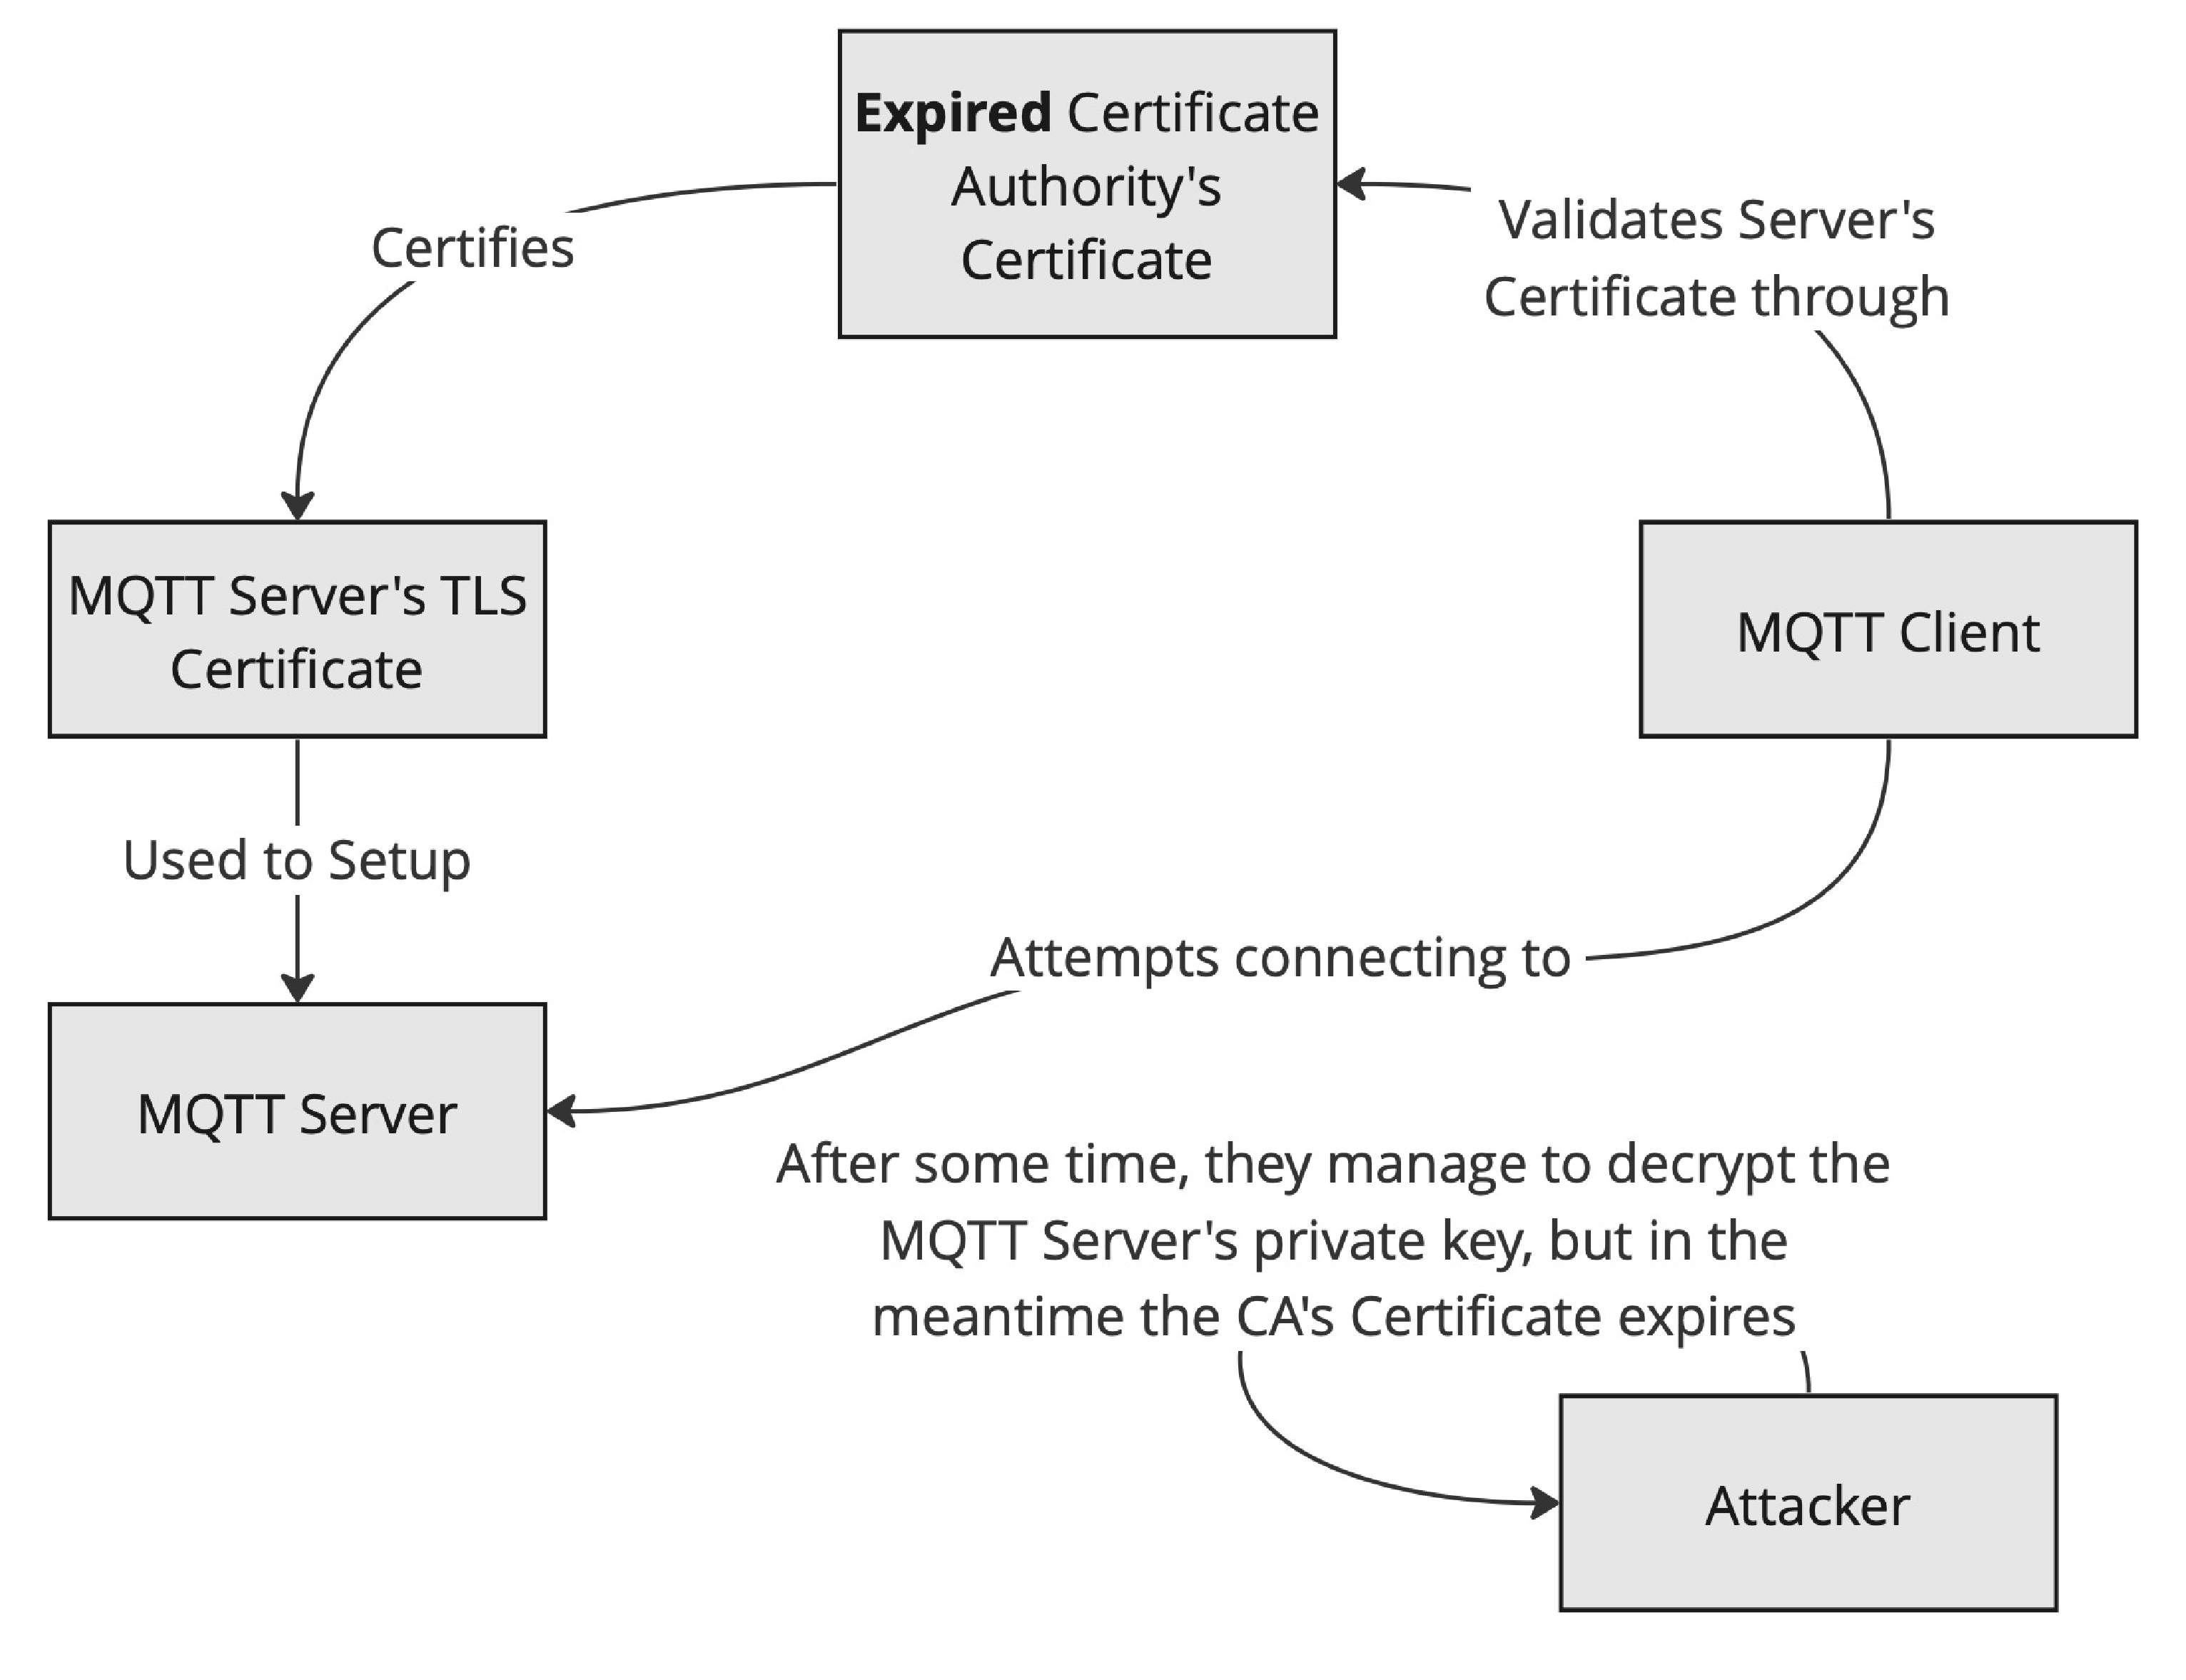
\includegraphics[width=12cm]{TC7}

\section{Test Case 8 - Certificate Extension}
This Test Case is set up by configuring the MQTT Broker Library with a valid TLS Certificate signed by the real Certificate Authority, though this Certificate has been signed by the CA for the MQTT Broker to use only as a Client Certificate towards other Brokers (in mTLS). The Tester Client connects to the server checking the Server TLS Certificate against the real Certificate Authority’s Certificate. The table of the Unit Test is as follows:

\begin{center}
\begin{tabular}{| p{6cm} | p{6cm} |}
\hline
Intruder Access Capabilities & The Intruder has access to a certificate belonging to the Server’s entity, but one that is used for TLS Client Authentication. \\
\hline
Intruder’s Attack description & The Intruder tries using the TLS Client Certificate to configure the MQTT Library as a MQTT Server, hence using the certificate as a TLS Server Certificate. \\
\hline
State of TLS Certificate & The TLS Certificate is rightfully authenticating the MQTT Server entity, but this TLS Certificate is not intended to be used for Server Authentication. \\
\hline
State of Certificate’s Signature & The signature is \textbf{\textit{valid}} \\
\hline
Assertion & The Library should \textbf{\textit{reject}} the connection when a client tries connecting to the MQTT Library configured with this certificate. \\
\hline
\end{tabular}
\end{center}

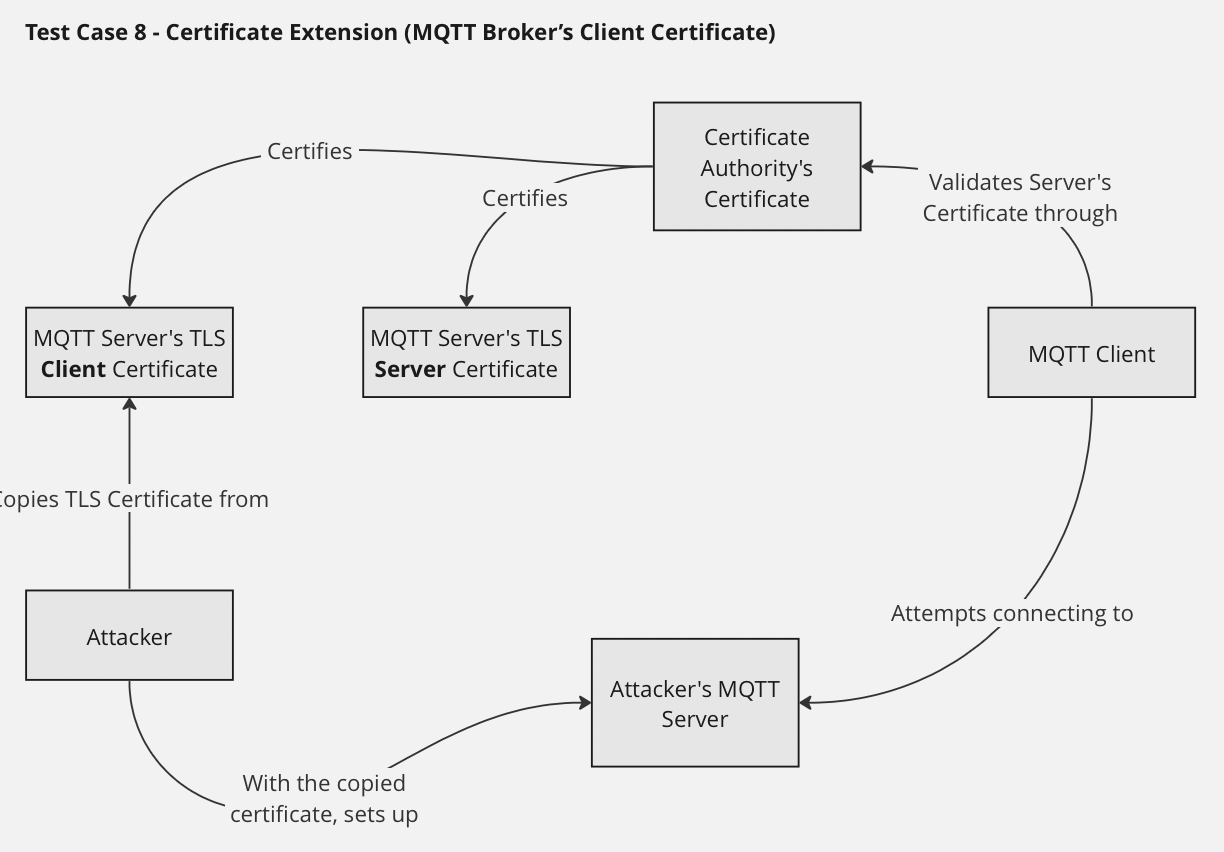
\includegraphics[width=13cm]{TC8}

\section{Test Case 9 - Longer Chain Of Trust Legal Connection}
This Test Case is set up by configuring the MQTT Broker Library with a valid TLS Certificate signed by the real Intermediate Certificate Authority, which in turn is signed by the real Root Certificate Authority. The Tester Client connects to the server checking the Server TLS Certificate against the real Root Certificate Authority’s Certificate. The table of the Unit Test is as follows:

\begin{center}
\begin{tabular}{| p{6cm} | p{6cm} |}
\hline
Intruder Access Capabilities & None \\
\hline
Intruder’s Attack description & This test case represents a happy path with no intruder attack and with a longer chain of trust (Root CA + Intermediate CA). \\
\hline
State of TLS Certificate & The TLS Certificate we use for this test is exactly the Server’s Certificate. (In this case, the Client connecting to the Server expects to receive a certificate signed by the Intermediate CA) \\
\hline
State of Certificate’s Signature & The signature is \textbf{\textit{valid}} \\
\hline
Assertion & The Library should \textbf{\textit{accept}} the connection when a client tries connecting to the MQTT Library configured with this certificate. \\
\hline
\end{tabular}
\end{center}

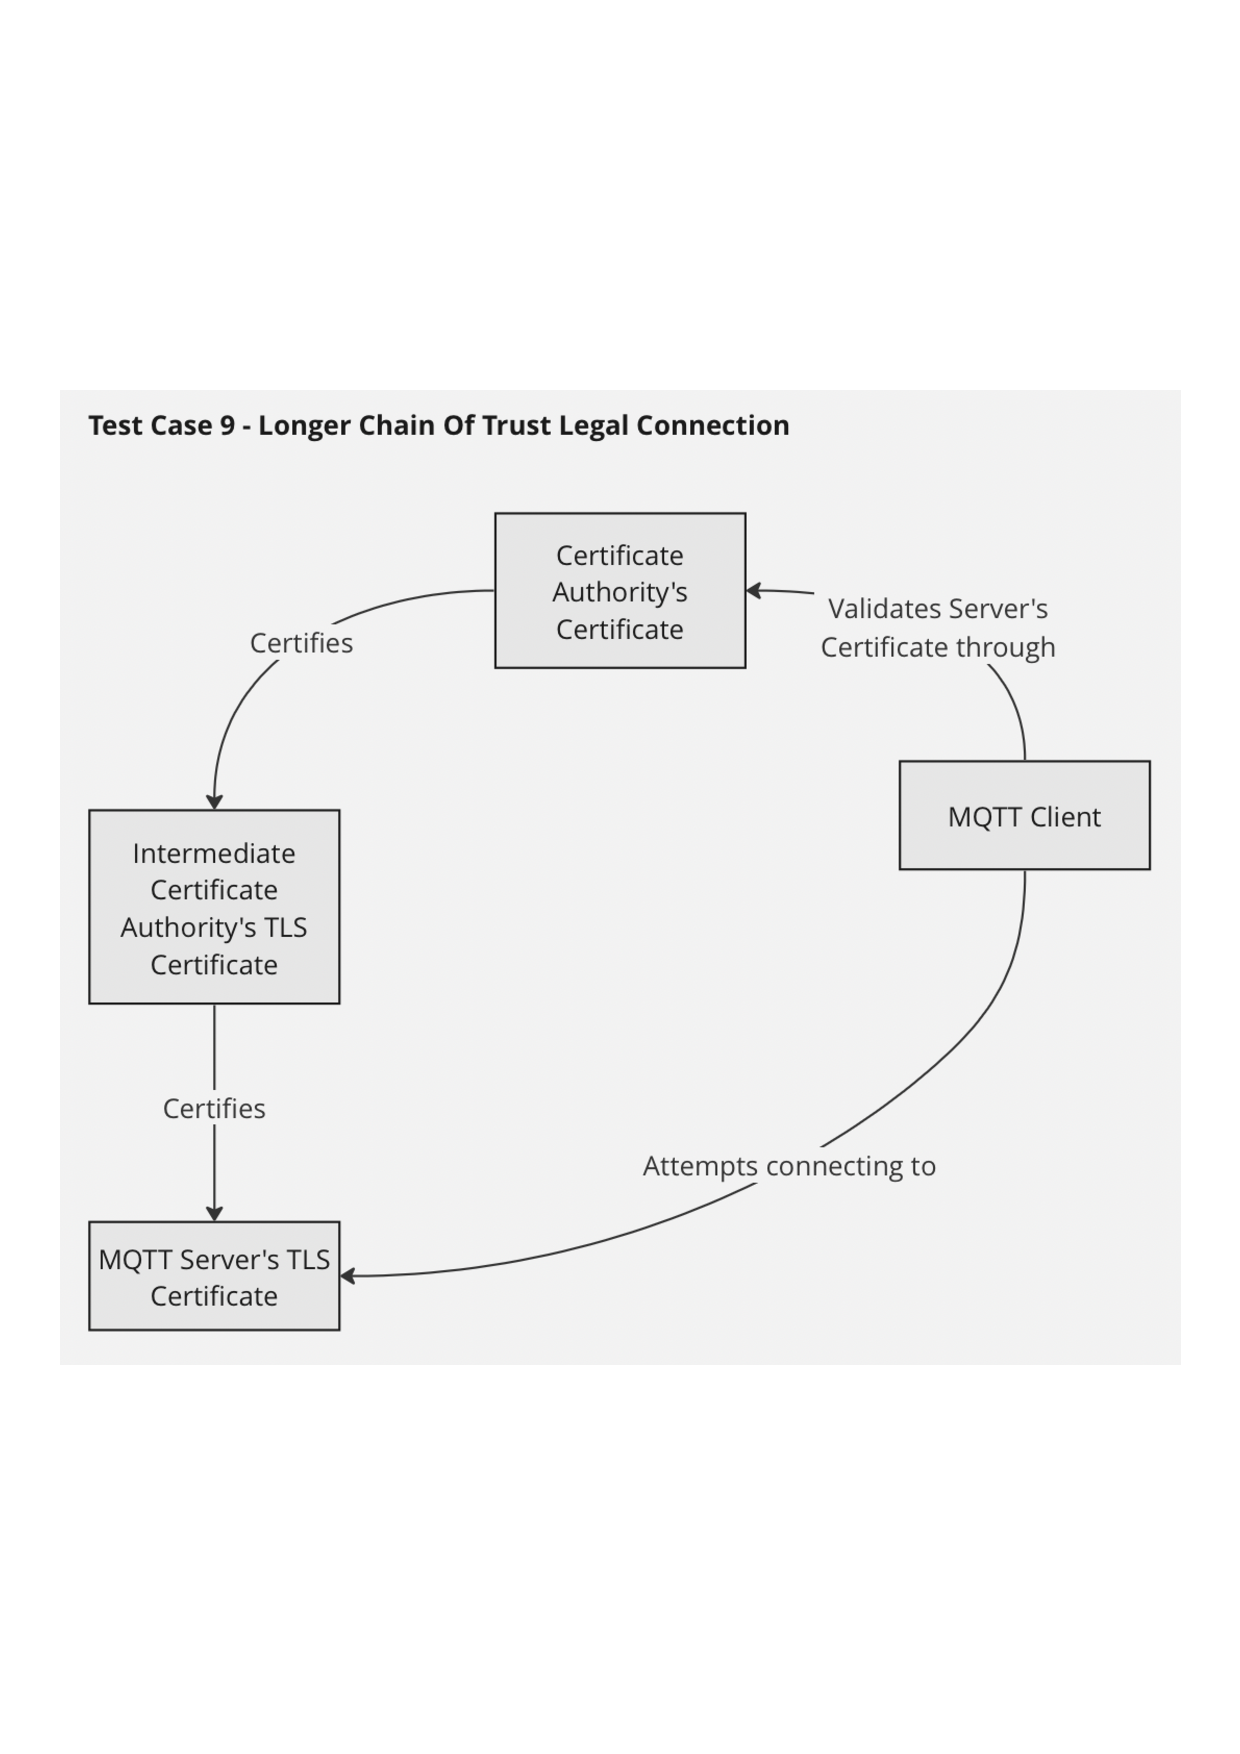
\includegraphics[width=11cm]{TC9}

\section{Test Case 10 - Altered Intermediate CA Common Name}
This Test Case is set up by configuring the MQTT Broker Library with a forged TLS Certificate signed by an altered Intermediate Certificate Authority, which in turn is signed by the real Root Certificate Authority. The intruder alters their Intermediate CA’s Common Name to pretend they are the real Intermediate CA, therefore the signature of the Intermediate CA is compromised. The Tester Client connects to the server checking the Server TLS Certificate against the real Root Certificate Authority’s Certificate. The table of the Unit Test is as follows:

\begin{center}
\begin{tabular}{| p{6cm} | p{6cm} |}
\hline
Intruder Access Capabilities & The Intruder owns an intermediate CA certificate signed by the Root CA. \\
\hline
Intruder’s Attack description & The Intruder alters its certificate Common Name, trying to trick the client into believing the Intruder is signed by the real Intermediate CA. \\
\hline
State of TLS Certificate & The TLS Certificate is imitating the Server Certificate, but it’s signed by the Attacker’s fake Certificate Authority. (In this case, the Client connecting to the Server expects to receive a certificate signed by the Intermediate CA) \\
\hline
State of Certificate’s Signature & The signature is \textbf{\textit{not}} valid \\
\hline
Assertion & The Library should \textbf{\textit{reject}} the connection when a client tries connecting to the MQTT Library configured with this certificate. \\
\hline
\end{tabular}
\end{center}

\newpage
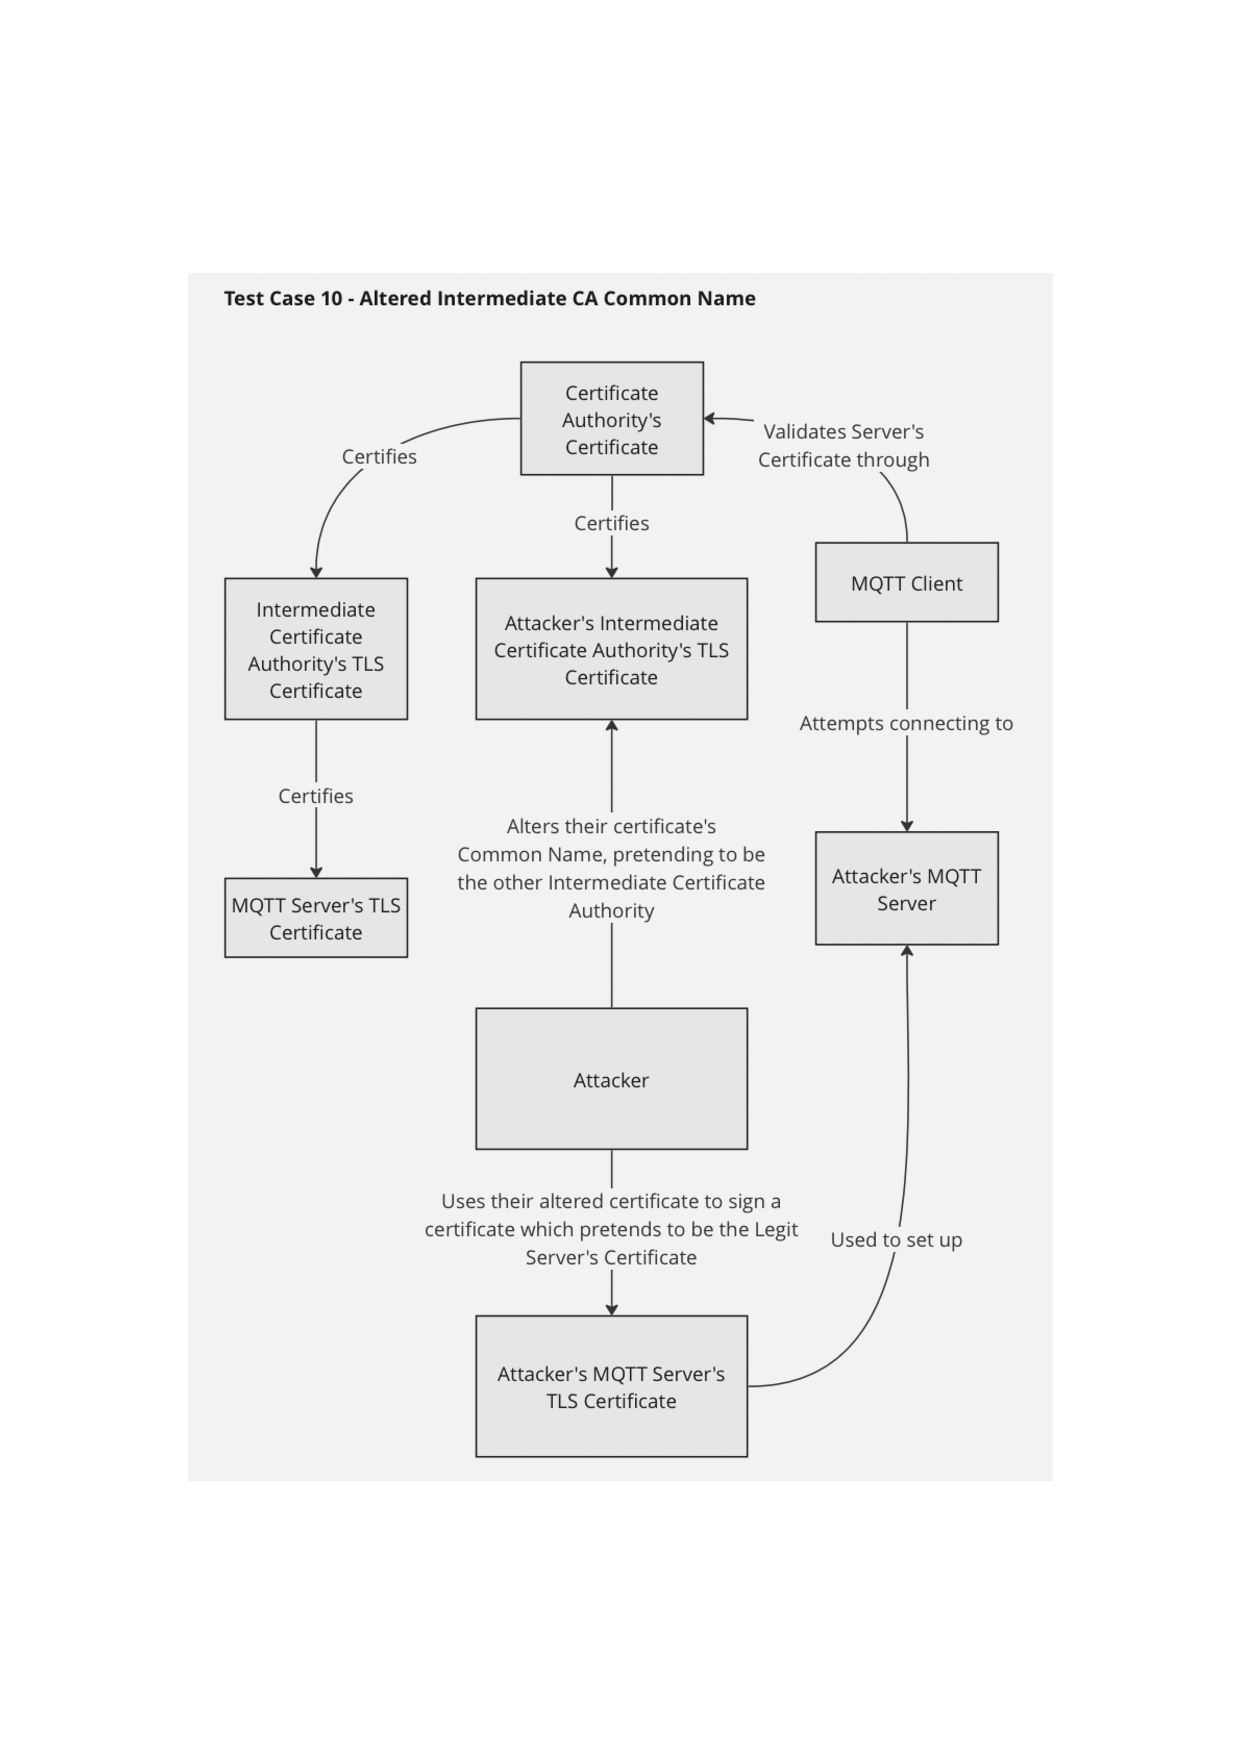
\includegraphics[width=13cm]{TC10}

\section{Test Case 11 - Altered Intermediate CA Public Key}
This Test Case is set up by configuring the MQTT Broker Library with a forged TLS Certificate signed by an altered Intermediate Certificate Authority, which in turn is signed by the real Root Certificate Authority. The intruder replaces the real Intermediate CA’s Public Key field contents with their own Public Key, to be able to decrypt the traffic easily, therefore the signature of the Intermediate CA is compromised. The Tester Client connects to the server checking the Server TLS Certificate against the real Root Certificate Authority’s Certificate. The table of the Unit Test is as follows:

\begin{center}
\begin{tabular}{| p{6cm} | p{6cm} |}
\hline
Intruder Access Capabilities & The Intruder owns the Intermediate CA’s Certificate. \\
\hline
Intruder’s Attack description & The Intruder alters the Intermediate CA’s Public Key field with their own Public Key, trying to trick the client into sending their traffic in a way that is easy to decrypt for the Intruder. \\
\hline
State of TLS Certificate & The TLS Certificate is imitating the Server Certificate, but it’s signed by the Attacker’s fake Certificate Authority. (In this case, the Client connecting to the Server expects to receive a certificate signed by the Intermediate CA) \\
\hline
State of Certificate’s Signature & The signature is \textbf{\textit{not}} valid \\
\hline
Assertion & The Library should \textbf{\textit{reject}} the connection when a client tries connecting to the MQTT Library configured with this certificate. \\
\hline
\end{tabular}
\end{center}

\newpage
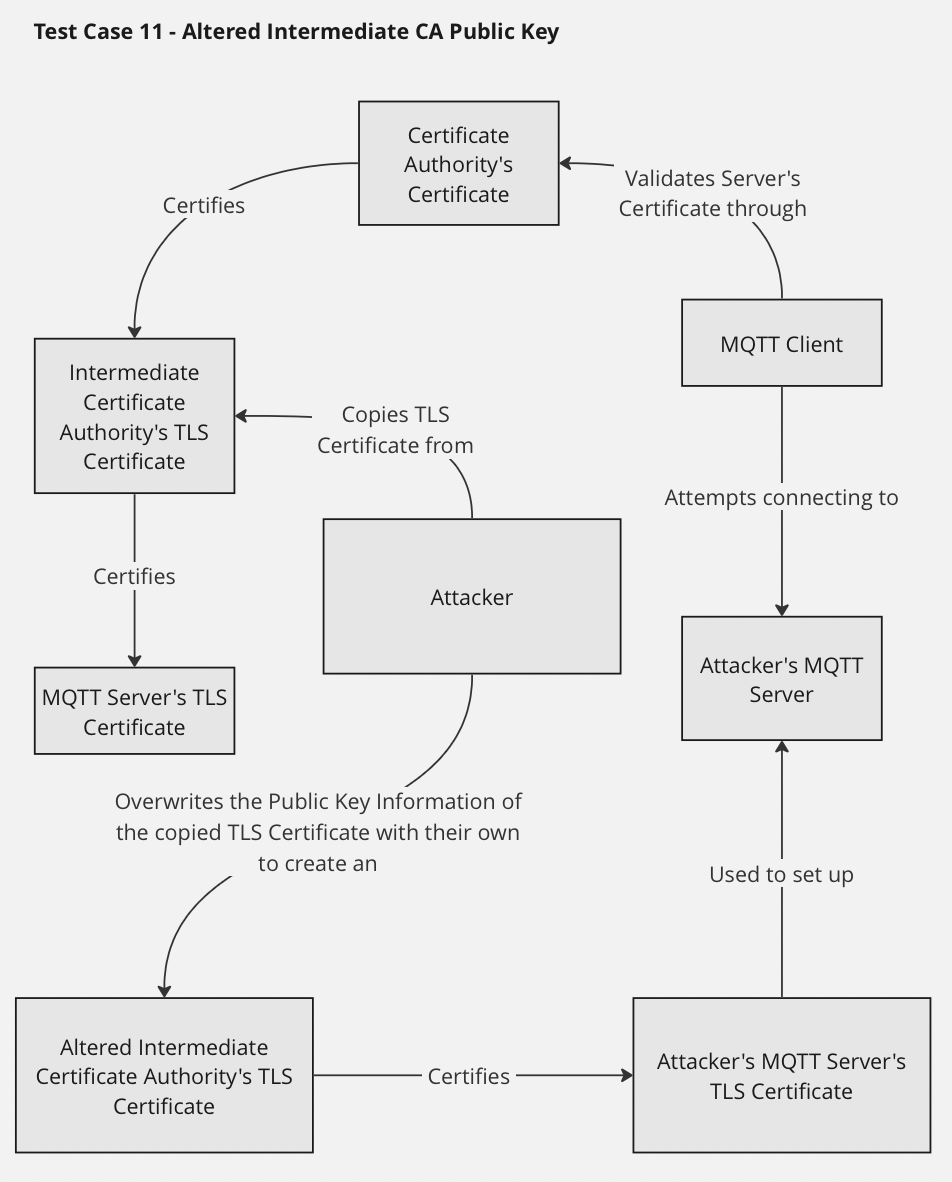
\includegraphics[width=13cm]{TC11}

\chapter{Developed Code}
The code developed for this Internship is used to setup the laboratory environment and to execute the Unit Tests for each library. For each file there will be the code snippet followed by an explanation of the code.

\section{TLS Certificates Generation Script}
\lstinputlisting[language=Bash]{snippets/setupCertificates.sh}
This script, `\textbf{setupCertificates.sh}', is the main piece of code which creates the certificates for all the actors involved in the above defined Unit Tests, using the OpenSSL library to do so. When executed, we need to pass as argument the IP address of the  MQTT Library Docker Container which will act as our MQTT Server. The reason we need this argument is that, when generating the certificates, we will need to specify this IP as the Server Certificate’s Common Name.
To start off, the script calls the subscript `\textbf{clean.sh}' to remove existing certificates and folders that we are going to create later. This is done in order to allow the script to be called multiple times if needed. The script then proceeds creating the following Certificate Authority folders:
\begin{itemize}
	\item ca: this is the Root Certificate Authority used to sign the MQTT Server’s TLS Certificate.
	\item second-level-ca: this is the Intermediate Certificate Authority, signed by the  Root CA and used to sign the MQTT Server’s TLS Certificate in the Test Case 9.
	\item expired-ca: this is a Root Certificate Authority which has been used to sign the MQTT Server’s TLS Certificate but is now expired.
	\item fake-ca: this is a Root Certificate Authority forged by the Attacker to look like the real Root CA.
	\item second-level-ca-2: this is an Intermediate Certificate Authority owned by the Attacker and signed by the Root CA. It is used by the Attacker in Test Case 10  to pretend to be the real Intermediate Certificate Authority.
	\item second-level-ca-alt1-common-name: this is the destination folder of the Attacker’s Intermediate Certificate Authority after they tampered with its Common Name field.
	\item second-level-ca-alt2-public-key: this is the destination folder of the altered  Intermediate Certificate Authority after the attacker tampered with its Public Key field. Used in Test Case 11.
\end{itemize}

The script then proceeds creating the following TLS Certificate folders:
\begin{itemize}
	\item server-certificate: this folder will contain the TLS Certificate belonging to the MQTT Server.
	\item attacker-certificate: this folder will contain the self-signed TLS Certificate belonging to the Attacker.
	\item alt1-common-name: this folder will contain the MQTT Server’s Altered TLS Certificate, after the attacker tampered with its Common Name field.
	\item alt2-expiration-date: this folder will contain the MQTT Server’s Altered TLS Certificate, after the attacker tampered with its Not Valid After field.
	\item alt3-public-key: this folder will contain the MQTT Server’s Altered TLS Certificate, after the attacker tampered with its Public Key field.
	\item alt4-expired-ca: this folder will contain the Attacker’s TLS Certificate signed by the expired Root CA.
	\item fake-chain-of-trust: this folder will contain the Attacker’s TLS Certificate signed by their Fake Root Certificate Authority.
	\item attacker-certificate-signed-by-altered-int-ca: this folder will contain the Attacker's Intermediate CA Altered TLS Certificates, for Test Case 10 (Altered CA's Common Name) and Test Case 11 (Altered CA's Public Key)
\end{itemize}

The script then generates, in order:
\begin{itemize}
	\item the Root Certificate Authority's Private Key and TLS self-signed Certificate:
	\begin{itemize}
		\item ca/ca.key
		\item ca/ca.pem
	\end{itemize}
	\item the Legit MQTT Server's Private Key:
	\begin{itemize}
		\item server-certificate/serverKey.pem
	\end{itemize}
	\item the Legit MQTT Server's TLS Certificate signed by the Root CA:
	\begin{itemize}
		\item server-certificate/serverCertificate.pem
	\end{itemize}
	\item the Legit MQTT Server's Private Key for usage as a Client:
	\begin{itemize}
		\item server-certificate/serverKeyAsClient.pem
	\end{itemize}
	\item the Legit MQTT Server's TLS Certificate for usage as a Client, signed by the Root CA:
	\begin{itemize}
		\item server-certificate/serverCertificateAsClient.pem
	\end{itemize}
	\item the Intermediate Certificate Authority's Private Key:
	\begin{itemize}
		\item second-level-ca/ca.key
	\end{itemize}
	\item the Intermediate Certificate Authority TLS Certificate signed by the Root CA:
	\begin{itemize}
		\item second-level-ca/ca.pem
	\end{itemize}
	\item the Legit MQTT Server's TLS Certificate signed by the Intermediate CA:
	\begin{itemize}
		\item server-certificate/serverCertificateSignedByIntermediate.pem
	\end{itemize}
	\item the concatenation of Root CA's and Intermediate CA's TLS Certificates:
	\begin{itemize}
		\item second-level-ca/ca-chain-of-trust.pem
	\end{itemize}
	\item the Attacker's Private Key and TLS self-signed Certificate:
	\begin{itemize}
		\item attacker-certificate/attackerKey.pem
		\item attacker-certificate/attackerCertificate.pem
	\end{itemize}
	\item the Attacker's Fake Root Certificate Authority's Private Key and TLS self-signed Certificate:
	\begin{itemize}
		\item fake-ca/ca.key
		\item fake-ca/ca.pem
	\end{itemize}
	\item the Attacker's TLS Certificate signed by the Fake Root CA:
	\begin{itemize}
		\item fake-chain-of-trust/attackerCertificate.pem
	\end{itemize}
	\item a second (different) Intermediate Certificate Authority's Private Key:
	\begin{itemize}
		\item second-level-ca-2/ca.key
	\end{itemize}
	\item the TLS Certificate of the second Intermediate CA, signed by the Root CA:
	\begin{itemize}
		\item second-level-ca-2/ca.pem
	\end{itemize}
	\item the Alteration 1 (Common Name) of the second Intermediate CA's TLS Certificate:
	\begin{itemize}
		\item second-level-ca-alt1-common-name/ca.der
	\end{itemize}
	\item the Attacker's TLS Certificate signed by the Altered Intermediate CA (Alteration 1):
	\begin{itemize}
		\item attacker-certificate-signed-by-altered-int-ca/attackerCertificate-alt1.pem
	\end{itemize}
	\item the concatenation of Root CA's and Altered Intermediate CA (Alteration 1)'s TLS Certificates:
	\begin{itemize}
		\item second-level-ca-alt1-common-name/ca-chain-of-trust.pem
	\end{itemize}
	\item the Alteration 2 (Public Key) of the second Intermediate CA's TLS Certificate:
	\begin{itemize}
		\item second-level-ca-alt2-public-key/ca.der
	\end{itemize}
	\item the Attacker's TLS Certificate signed by the Altered Intermediate CA (Alteration 2):
	\begin{itemize}
		\item attacker-certificate-signed-by-altered-int-ca/attackerCertificate-alt2.pem
	\end{itemize}
	\item the concatenation of Root CA's and Altered Intermediate CA (Alteration 2)'s TLS Certificates:
	\begin{itemize}
		\item second-level-ca-alt2-public-key/ca-chain-of-trust.pem
	\end{itemize}
	\item the Alteration 1 (Common Name) of the Legit MQTT Server's TLS Certificate:
	\begin{itemize}
		\item alt1-common-name/attackerCertificate.der
	\end{itemize}
	\item the Alteration 2 (Expiration Date) of the Legit MQTT Server's TLS Certificate:
	\begin{itemize}
		\item alt2-expiration-date/attackerCertificate.der
	\end{itemize}
	\item the Alteration 3 (Public Key) of the Legit MQTT Server's TLS Certificate:
	\begin{itemize}
		\item alt3-public-key/attackerCertificate.der
	\end{itemize}
	\item the Expired Root CA's TLS Certificate:
	\begin{itemize}
		\item expired-ca/ca.pem
	\end{itemize}
	\item the Attacker's TLS Certificate signed by the Expired CA:
	\begin{itemize}
		\item alt4-expired-ca/attackerCertificate.der
	\end{itemize}

Lastly, the script converts back to `\textbf{.pem}' all the certificates that were saved in `\textbf{.der}' extension by the alteration scripts.
\end{itemize}
\section{TLS Certificate Common Name Alteration Script}
\lstinputlisting[language=Python]{snippets/alterCommonName.py}
Because this script is used to alter both the Legit MQTT Server's TLS Certificate and the second Intermediate CA's TLS Certificate, the script is designed to have 3 inputs:
\begin{itemize}
	\item Path of the certificate to be altered.
	\item Path of the destination where the altered certificate will be saved.
	\item Path of the reference certificate that will be used to copy and paste the Common Name from.
\end{itemize}
The script uses the `\textbf{pyasn1}' , `\textbf{pyasn1\_modules}' and `\textbf{sys}' libraries to:
\begin{enumerate}
	\item Read the certificate to be altered and the reference certificate from disk.
	\item Decode the certificate to be altered and the reference certificate, from ASN1-base64-encoded data to a Dictionary data structure.
	\item Overwrite the \textbf{Common Name} of the certificate to be altered with the \textbf{Common Name} of the reference Certificate.
	\item Encode the resulting Altered Certificate from a Dictionary data structure to a ASN1-base64-encoded data.
	\item Save the Altered Certificate on disk.
\end{enumerate}

\section{TLS Certificate Expiration Date Alteration Script}
\lstinputlisting[language=Python]{snippets/alterExpirationDate.py}
The script uses the `\textbf{pyasn1}' , `\textbf{pyasn1\_modules}' and `\textbf{sys}' libraries to:
\begin{enumerate}
	\item Read the certificate to be altered (`\textbf{server-certificate/serverCertificate.der}') from disk.
	\item Decode the certificate to be altered from ASN1-base64-encoded data to a Dictionary data structure.
	\item Change the validity range (`\textbf{Not Valid Before}' and `\textbf{Not Valid After}' fields) to a range that contains the current date, for example in the script it's changed to years 2001 until 2040.
	\item Encode the resulting Altered Certificate from a Dictionary data structure to a ASN1-base64-encoded data.
	\item Save the Altered Certificate on disk.
\end{enumerate}

\section{TLS Certificate Public Key Alteration Script}
\lstinputlisting[language=Python]{snippets/alterPublicKey.py}
Because this script is used to alter both the Legit MQTT Server's TLS Certificate and the Intermediate CA's TLS Certificate, the script is designed to have 3 inputs:
\begin{itemize}
	\item Path of the certificate to be altered.
	\item Path of the destination where the altered certificate will be saved.
	\item Path of the reference certificate that will be used to copy and paste the Common Name from.
\end{itemize}
The script uses the `\textbf{pyasn1}' , `\textbf{pyasn1\_modules}' and `\textbf{sys}' libraries to:
\begin{enumerate}
	\item Read the certificate to be altered and the reference certificate from disk.
	\item Decode the certificate to be altered and the reference certificate, from ASN1-base64-encoded data to a Dictionary data structure.
	\item Overwrite the \textbf{Public Key} of the certificate to be altered with the \textbf{Public Key} of the reference Certificate.
	\item Encode the resulting Altered Certificate from a Dictionary data structure to a ASN1-base64-encoded data.
	\item Save the Altered Certificate on disk.
\end{enumerate}

\section{TLS Certificate Keystores Generation Script}
\lstinputlisting[language=Bash]{snippets/setupKeystores.sh}
Some of the tested MQTT Libraries work with Java Keystores (JKS) instead of retrieving the TLS Certificates from absolute paths. Therefore this script is designed to save the TLS Certificates generated by the `\textbf{setupCertificates.sh}' script into Java Keystores.
More specifically, the script applies these steps to the certificates and private keys of each Test Case:
\begin{enumerate}
	\item Save a `\textbf{.p12}' keystore containing the Server's Certificate and Private Key, using the `\textbf{openssl pkcs12}' tool.
	\item Convert the `\textbf{.p12}' keystore to a `\textbf{.jks}' keystore using the \textbf{default-jre}'s `\textbf{keytool}' command.
\end{enumerate}
All the derived keystores are saved in the `keystores' folder.

\section{MQTT Client Tester Script}
\lstinputlisting[language=Bash]{snippets/testMQTTBroker.sh}
The Tester (MQTT Client) uses a Tester Script named `\textbf{testMQTTBroker.sh}', invoking a Mosquitto Command-Line Interface distribution subscription command to connect to the MQTT Server set up by the Test Environment. The Tester Script then checks if the subscription was active (if exit code is 0) and prints a line on \textbf{stdout} that represents the Unit Test Result.
The Tester Script also accepts an optional argument to specify a Certificate Authority TLS Certificate path to use to connect to the MQTT Server. This is used mainly for \textbf{Test Case 7}, where the reference CA TLS Certificate to use must be the expired one.
\section{Library Tester Script}
\lstinputlisting[language=Bash]{snippets/runTests.sh}
For each library an automated Tester Script has been developed. The script is designed to loop through the Test Cases, and for each test case the script will:
\begin{enumerate}
	\item Configure the MQTT Server Docker Container with the Broker Configuration of the current Test Case.
	\item Restart the MQTT Server Docker Container
	\item Command the MQTT Client Docker Container to try connecting to the MQTT Server using the MQTT Client Tester Script (`\textbf{testMQTTBroker.sh}')
	\item Proceed to the next Test Case
\end{enumerate}
The automated script works only if, before executing it, both the MQTT Server and MQTT Client Docker Containers are running.

\section{Docker Test Environment}
\subsection{MQTT Client Tester Image}
For the Docker Test Environment, the main piece of work was to setup the MQTT Client Tester Docker Container Image. The code used for the generation of this Image can be found in the following Dockerfile:
\lstinputlisting{snippets/tester-image-dockerfile}

The Dockerfile is based on the Linux Debian operating system image. It stores all its files in the folders `\textbf{/app}' and `\textbf{/app/src}'. The main files that are copied in these folders are:
\begin{itemize}
	\item setupCertificates.sh
	\item setupKeystores.sh
	\item testMQTTBroker.sh
	\item requirements.txt (configuration file to install python package dependencies)
	\item Test configurations for: \textbf{EMQX}, \textbf{HiveMQ} and \textbf{Mosquitto}
	\item Automated scripts to run all Test Cases for: \textbf{EMQX}, \textbf{HiveMQ}, \textbf{Mosquitto}, \textbf{Aedes} and \textbf{Moquette}
\end{itemize}

The Dockerfile also installs all the tools and libraries needed to run the tests:
\begin{itemize}
	\item python
	\item pip
	\item python virtual environment
	\item git
	\item openssl
	\item mosquitto
	\item mosquitto-clients
	\item default-jre
\end{itemize}
\subsection{Moquette MQTT Server Image}
There was no official Moquette Docker Container Image on Docker Hub, so our work included also the creation of a MQTT Server Docker Container Image which runs Moquette on startup.
The code used for the generation of this Image can be found in the following Dockerfile:
\lstinputlisting{snippets/moquette-image-dockerfile}

This Dockerfile is also based on the Linux Debian operating system image. It stores all its files in the folder `\textbf{/app/src/moquette}'. This folder contains a pre-compiled version of the Moquette MQTT Broker library.
The Dockerfile also installs all the dependencies needed by Moquette to run the MQTT Server:
\begin{itemize}
	\item openssl
	\item default-jre
\end{itemize}
Lastly, the Dockerfile runs on startup the script `\textbf{/app/src/moquette/bin/moquette.sh}'
\subsection{Aedes MQTT Server Image}
The official Aedes Docker Container Image found on Docker Hub had a very complex Container setup that used Docker Volumes to setup the configuration of the library. Because this procedure was not fitting our means of testing, we decided to create a custom MQTT Server Docker Container Image which runs Aedes on startup.

The code used for the generation of this Image can be found in the following Dockerfile:
\lstinputlisting{snippets/aedes-image-dockerfile}

This Dockerfile is also based on the Linux Debian operating system image. It stores all its files in the folder `\textbf{/app/src}'. This folder contains:
\begin{itemize}
	\item the Aedes test configurations needed to run each Test Case
	\item a `\textbf{run.sh}' script which simply runs aedes-cli getting the configuration from the path `\textbf{/app/src/config/conf.js}'
\end{itemize}
The Dockerfile also installs all the dependencies needed to run Aedes' MQTT Server, and it installs the latest version of Aedes itself.
The dependencies are:
\begin{itemize}
	\item openssl
	\item default-jre
	\item npm
\end{itemize}
Lastly, the Dockerfile runs on startup the above mentioned script `\textbf{run.sh}'.

\chapter{Test Results}
\section{Tested MQTT Libraries}
These are the Libraries that were subjected to Unit Testing and their respective version:

\begin{center}
\begin{tabular}{| p{6cm} | p{6cm} |}
\hline
\textbf{Library Name} & \textbf{Tested Version} \\
\hline
Mosquitto & 2.0.18 \\
\hline
HiveMQ Community Edition & 2023.9 \\
\hline
Aedes & 0.8.0 \\
\hline
Moquette & 0.18 \\
\hline
EMQX & 5.3.0 \\
\hline
RouterOS & CHR (6.49.10 Long-term) \\
\hline
\end{tabular}
\end{center}

All the Libraries except RouterOS have been set up as MQTT Broker and have been interacted with using the Mosquitto command line tools as MQTT Tester Client. On the other hand, RouterOS is a Library that enables MQTT connection in the form of Client-only up until version \textbf{v7.4beta4}. Therefore, RouterOS has been submitted to the same Test Suite as the other Libraries, except the Client connection was made by the tested Library itself, and the MQTT Tester Broker we chose was Mosquitto.

\newpage
\section{Result Table}
The Test Results for the tested Libraries can be found in the following tables. A tick `\cmark' represents a positive test outcome, a cross `\xmark' represents a failed test outcome.

\begin{flushleft}
\begin{tabular}{| p{2cm} | p{1.5cm} | p{1.5cm} | p{1.5cm} | p{1.5cm} | p{1.5cm} | p{1.5cm} |}
\hline
 & \multicolumn{3}{|c|}{\bf Chain of Trust} & \bf Host- name & \bf Exp. Date & \bf Public Key \\
\hline
\bf Library Name & \bf Test Case 1 & \bf Test Case 2 & \bf Test Case 3 & \bf Test Case 4 & \bf Test Case 5 & \bf Test Case 6 \\
\hline
Mosquitto & \cmark & \cmark & \cmark & \cmark & \cmark & \cmark  \\
\hline
HiveMQ Community Edition & \cmark & \cmark & \cmark & \cmark & \cmark & \cmark  \\
\hline
Aedes & \cmark & \cmark & \cmark & \cmark & \cmark & \cmark  \\
\hline
Moquette & \cmark & \cmark & \cmark & \cmark & \cmark & \cmark  \\
\hline
EMQX & \cmark & \cmark & \cmark & \cmark & \cmark & \cmark  \\
\hline
RouterOS & \cmark & \cmark & \cmark & \cmark & \cmark & \cmark  \\
\hline
\end{tabular}
\end{flushleft}

\begin{flushleft}
\begin{tabular}{| p{2cm} | p{1.5cm} | p{1.5cm} | p{1.5cm} | p{1.5cm} | p{1.5cm} |}
\hline
 & \bf Exp. Date & \bf Cert. Exten- sions & \bf Chain of trust & \bf Host- name & \bf Public Key \\
\hline
\bf Library Name & \bf Test Case 7 & \bf Test Case 8 & \bf Test Case 9 & \bf Test Case 10 & \bf Test Case 11 \\
\hline
Mosquitto & \cmark & \cmark & \cmark & \cmark & \cmark \\
\hline
HiveMQ Community Edition & \cmark & \cmark & \cmark & \cmark & \cmark \\
\hline
Aedes & \cmark & \cmark & \cmark & \cmark & \cmark \\
\hline
Moquette & \cmark & \cmark & \cmark & \cmark & \cmark \\
\hline
EMQX & \cmark & \cmark & \cmark & \cmark & \cmark \\
\hline
RouterOS & \cmark & \cmark & \cmark & \cmark & \cmark \\
\hline
\end{tabular}
\end{flushleft}

\subsection{Test Case 1 - Legal Connection}

In this Test Case we expected the Libraries to correctly accept the connection of our MQTT Tester Client, since the TLS Certificates used were all valid. All the Libraries passed this test, since all Libraries accepted our MQTT Tester Client connection.
RouterOS passed this test too, since it correctly connected to the Mosquitto Broker.

\subsection{Test Case 2 - Self Signed Attacker}
\subsection{Test Case 3 - Self Signed Attacker's Fake CA}
\subsection{Test Case 4 - Alteration 1 (Common Name)}
\subsection{Test Case 5 - Alteration 2 (Expiration Date)}
\subsection{Test Case 6 - Alteration 3 (Public Key)}
\subsection{Test Case 7 - Expired CA (Alteration 4)}
\subsection{Test Case 8 - Certificate Extension}
\subsection{Test Case 9 - Longer Chain Of Trust Legal Connection}
\subsection{Test Case 10 - Altered Intermediate CA Common Name}
\subsection{Test Case 11 - Altered Intermediate CA Public Key}

\chapter{Conclusion}
The development of the Unit Tests presented in this Internship Report allowed us to assert the security of the tested MQTT Broker Libraries and RouterOS CHR Operating System, which all passed the entirety of the developed Test Suite. Therefore, the results presented in Chapters 7 and 9 represent a validation of the TLS security requirements of the tested software.
Furthermore, the developed Test Suite and Laboratory Environment enables us for future monitoring of the TLS security requirements of new versions of the tested libraries, or of additional MQTT Broker Libraries altogether.

\backmatter
\cleardoublepage
\phantomsection % Give this command only if hyperref is loaded
\addcontentsline{toc}{chapter}{\bibname}

\printbibliography

\end{document}